

  \begin{figure}[h]
    \centering
    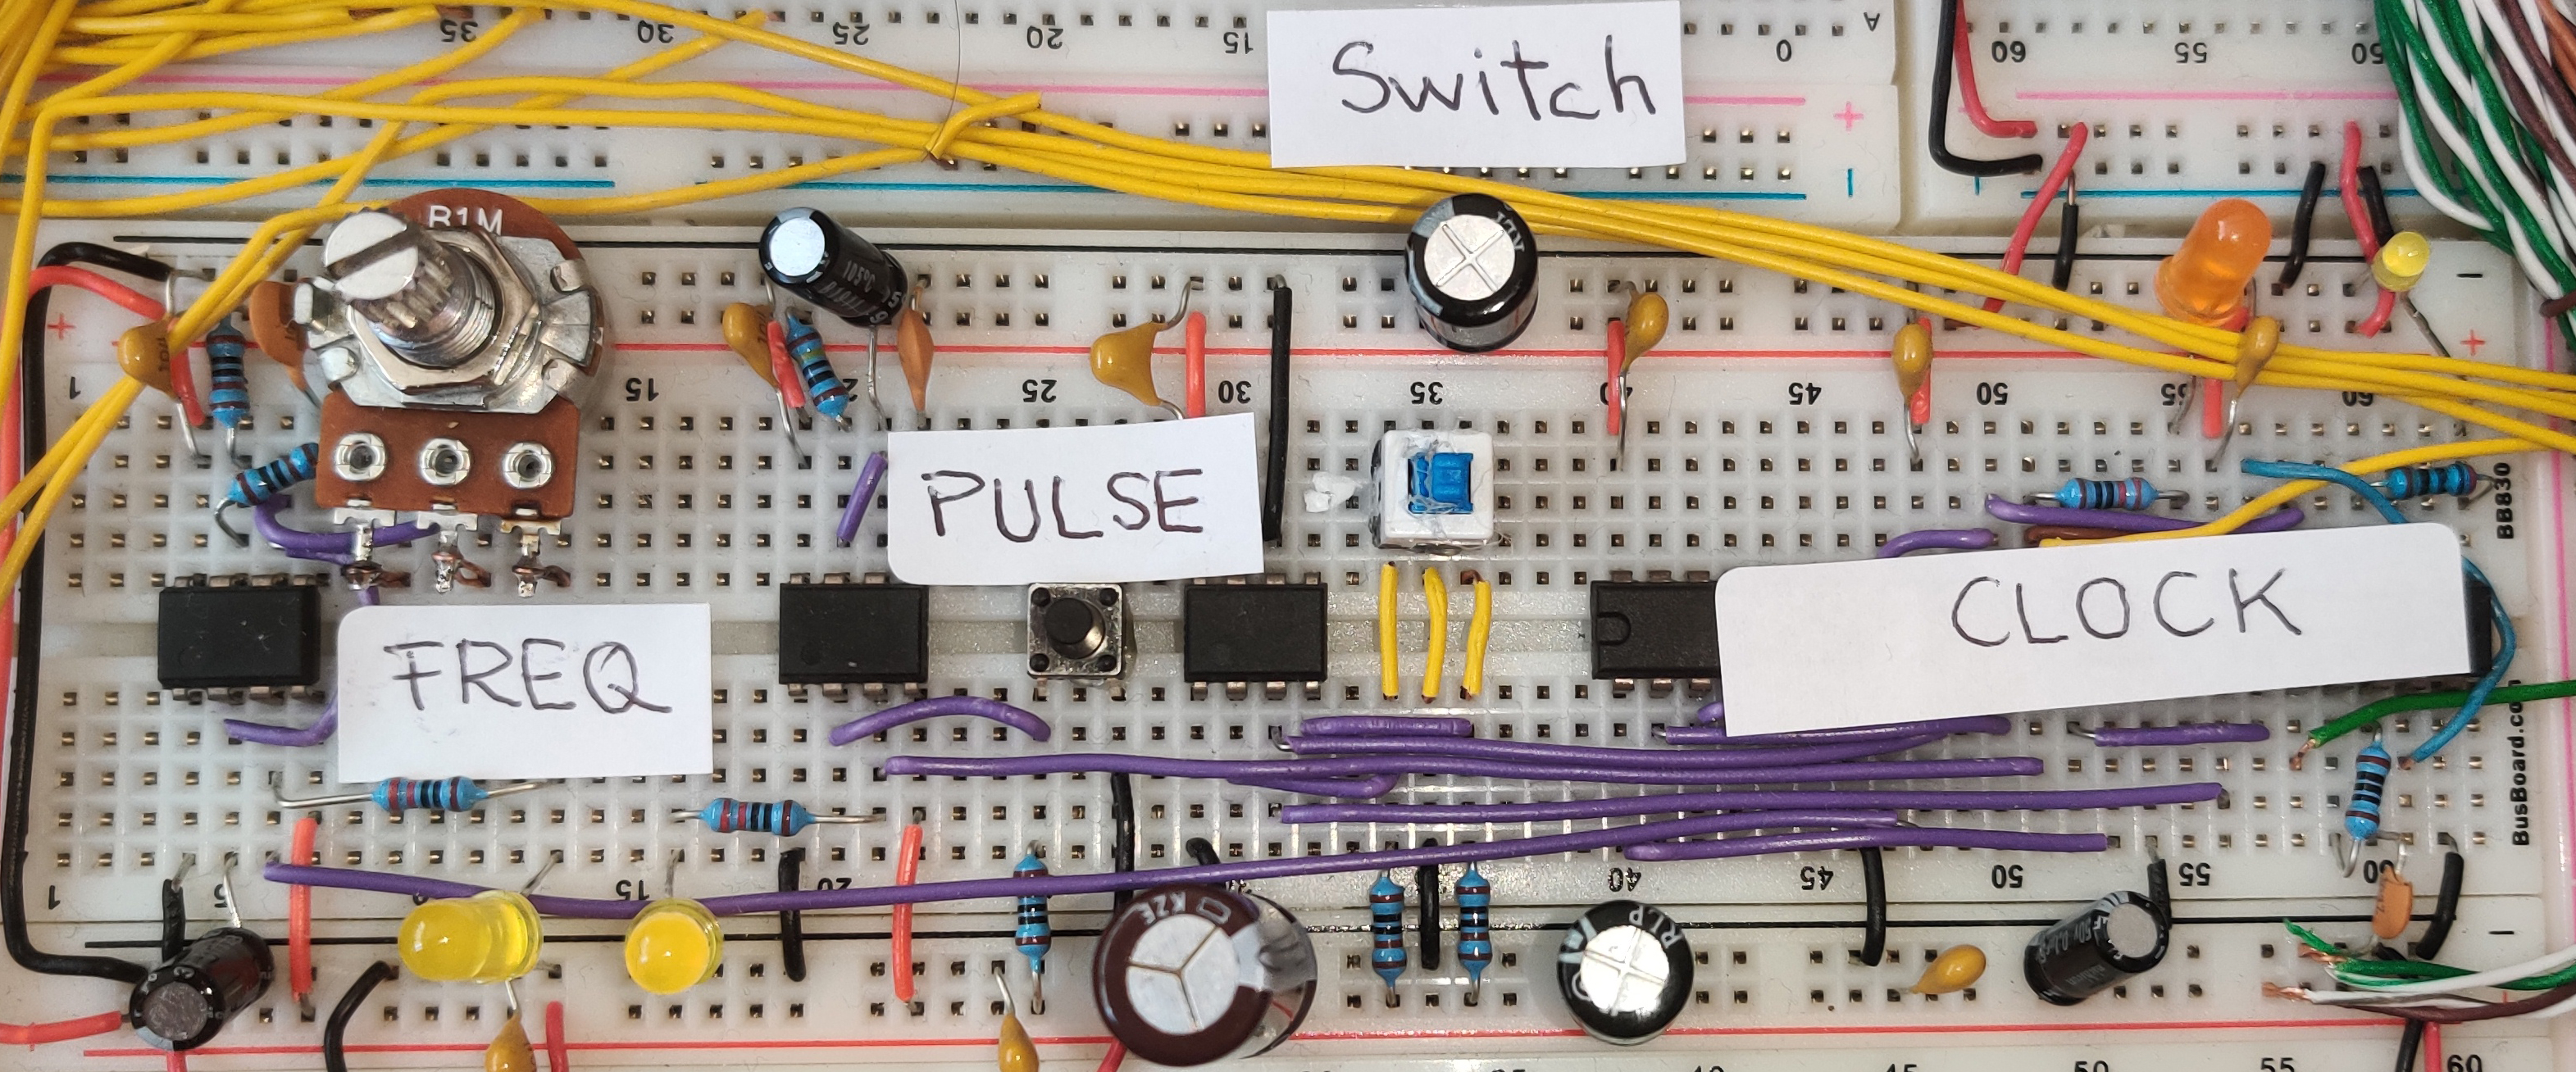
\includegraphics[scale=0.1]{comp/clock}
    \caption{Clock implementation}
    \label{clock-i}
  \end{figure}

  \begin{figure}[h]
    \centering
    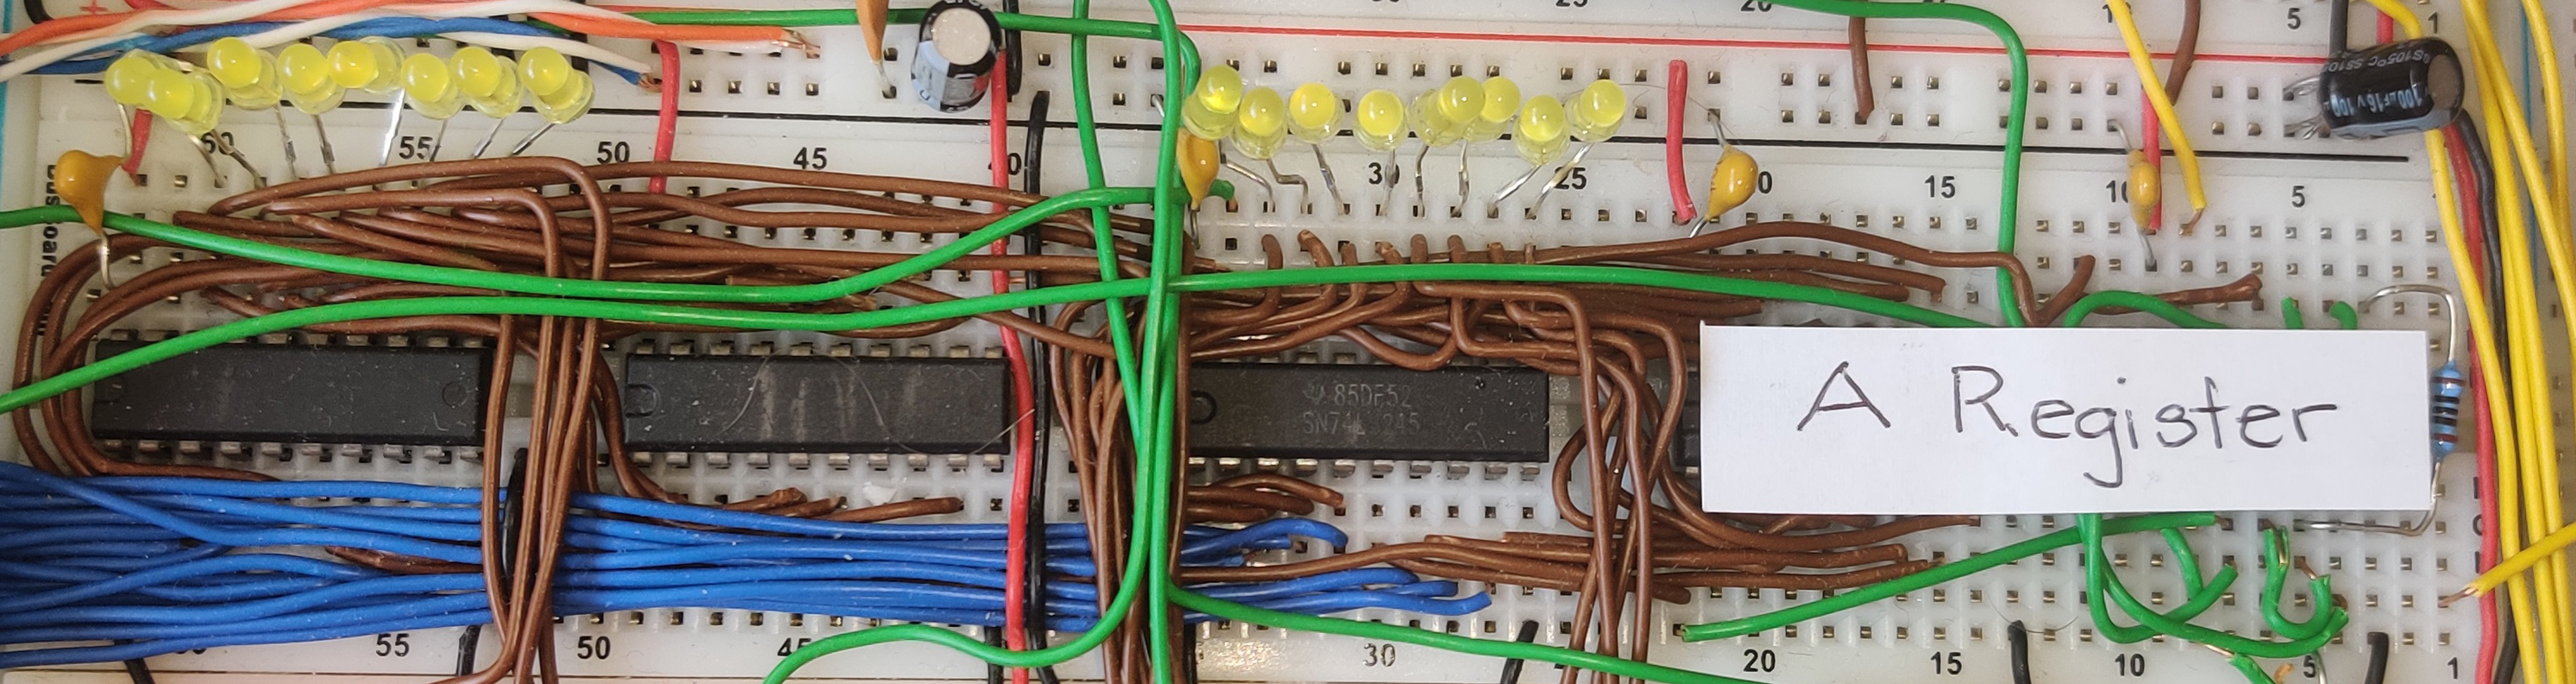
\includegraphics[scale=0.1]{comp/a-reg}
    \caption{A register implementation}
    \label{a-reg-i}
  \end{figure}

  \begin{figure}[h]
    \centering
    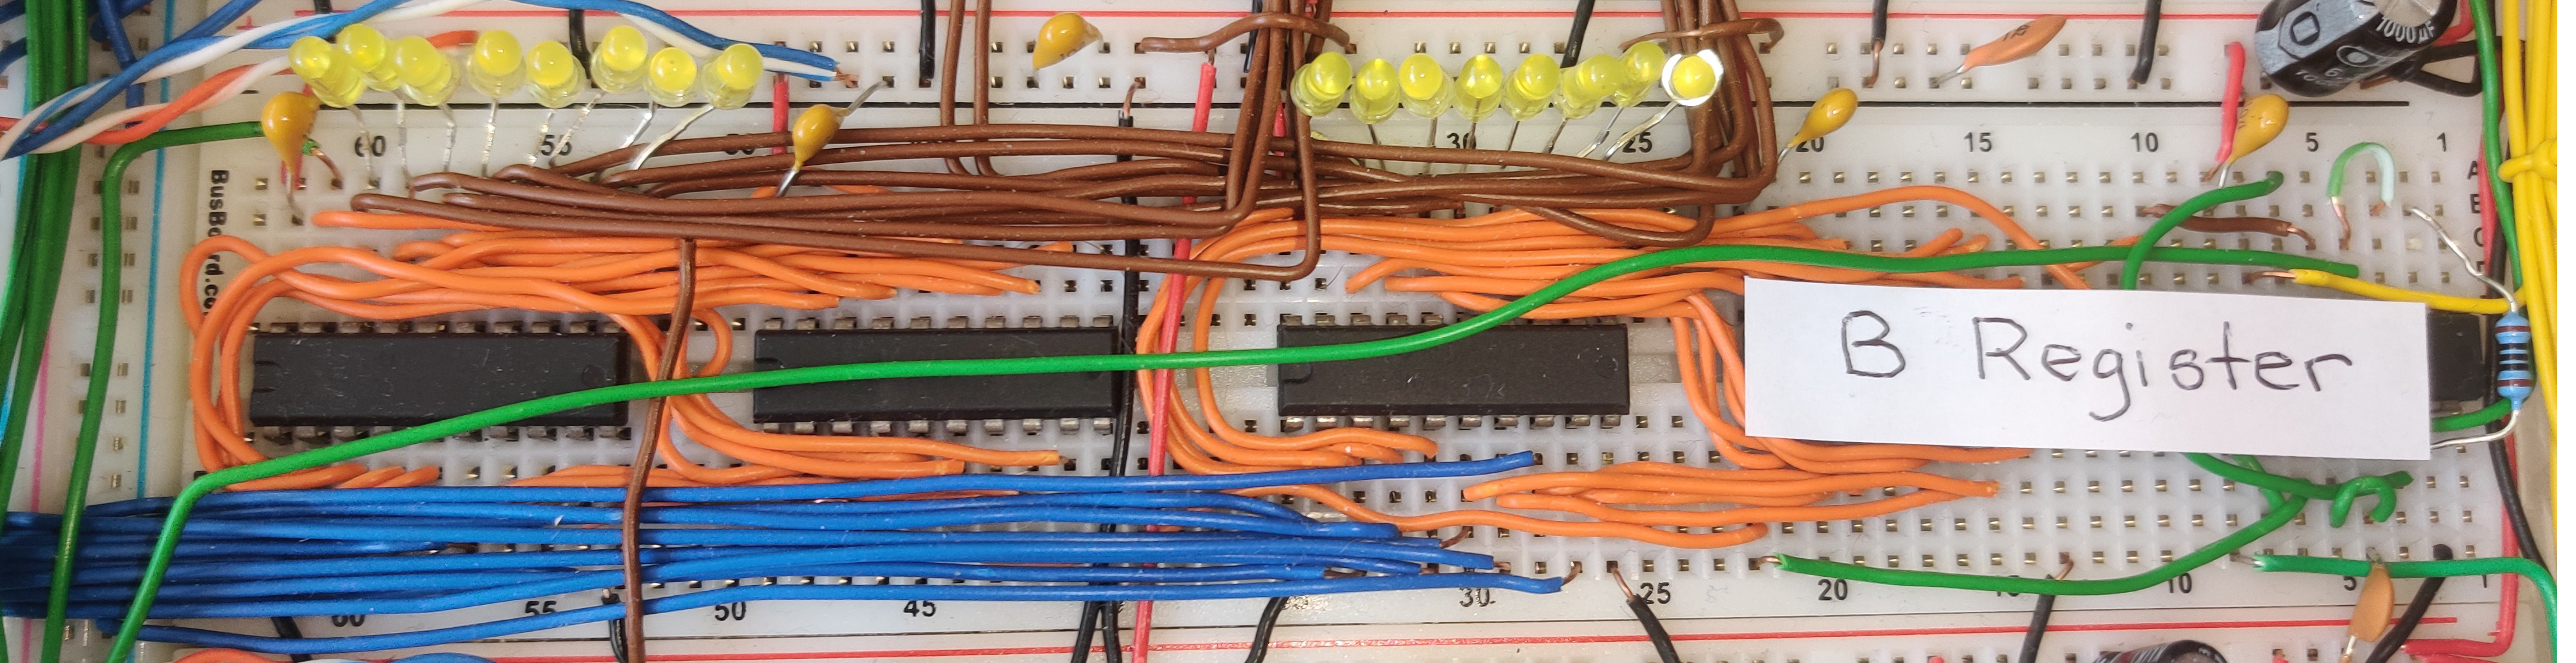
\includegraphics[scale=0.1]{comp/b-reg}
    \caption{B register implementation}
    \label{b-reg-i}
  \end{figure}

  \begin{figure}[h]
    \centering
    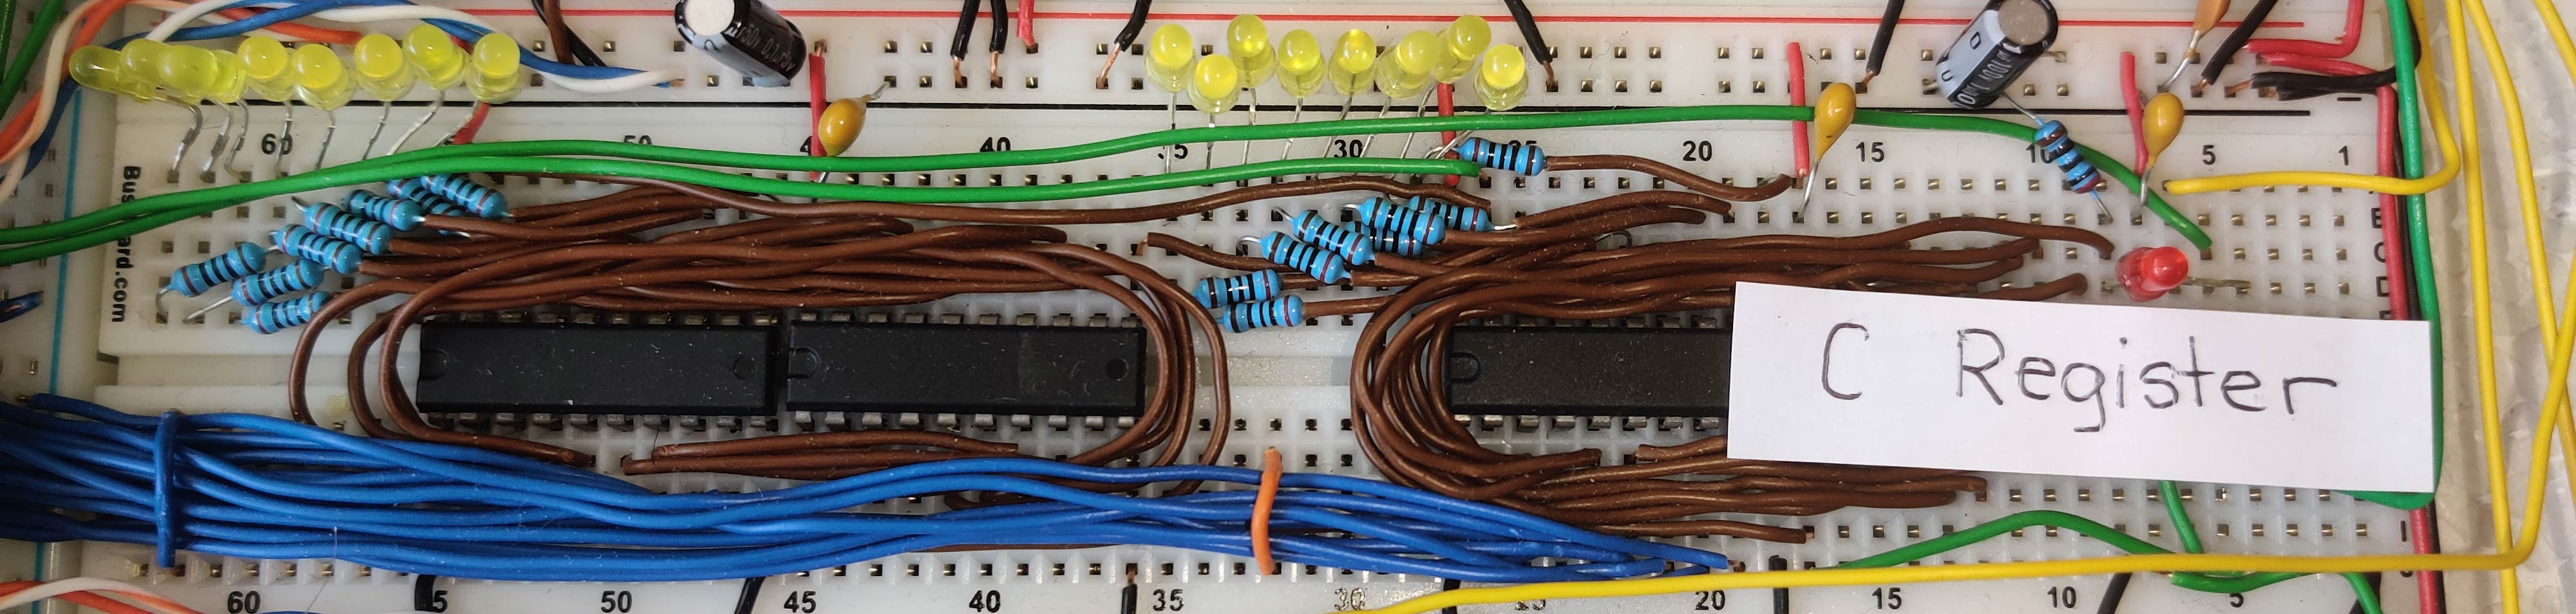
\includegraphics[scale=0.1]{comp/c-reg}
    \caption{C register implementation}
    \label{c-reg-i}
  \end{figure}

  \begin{figure}[h]
    \centering
    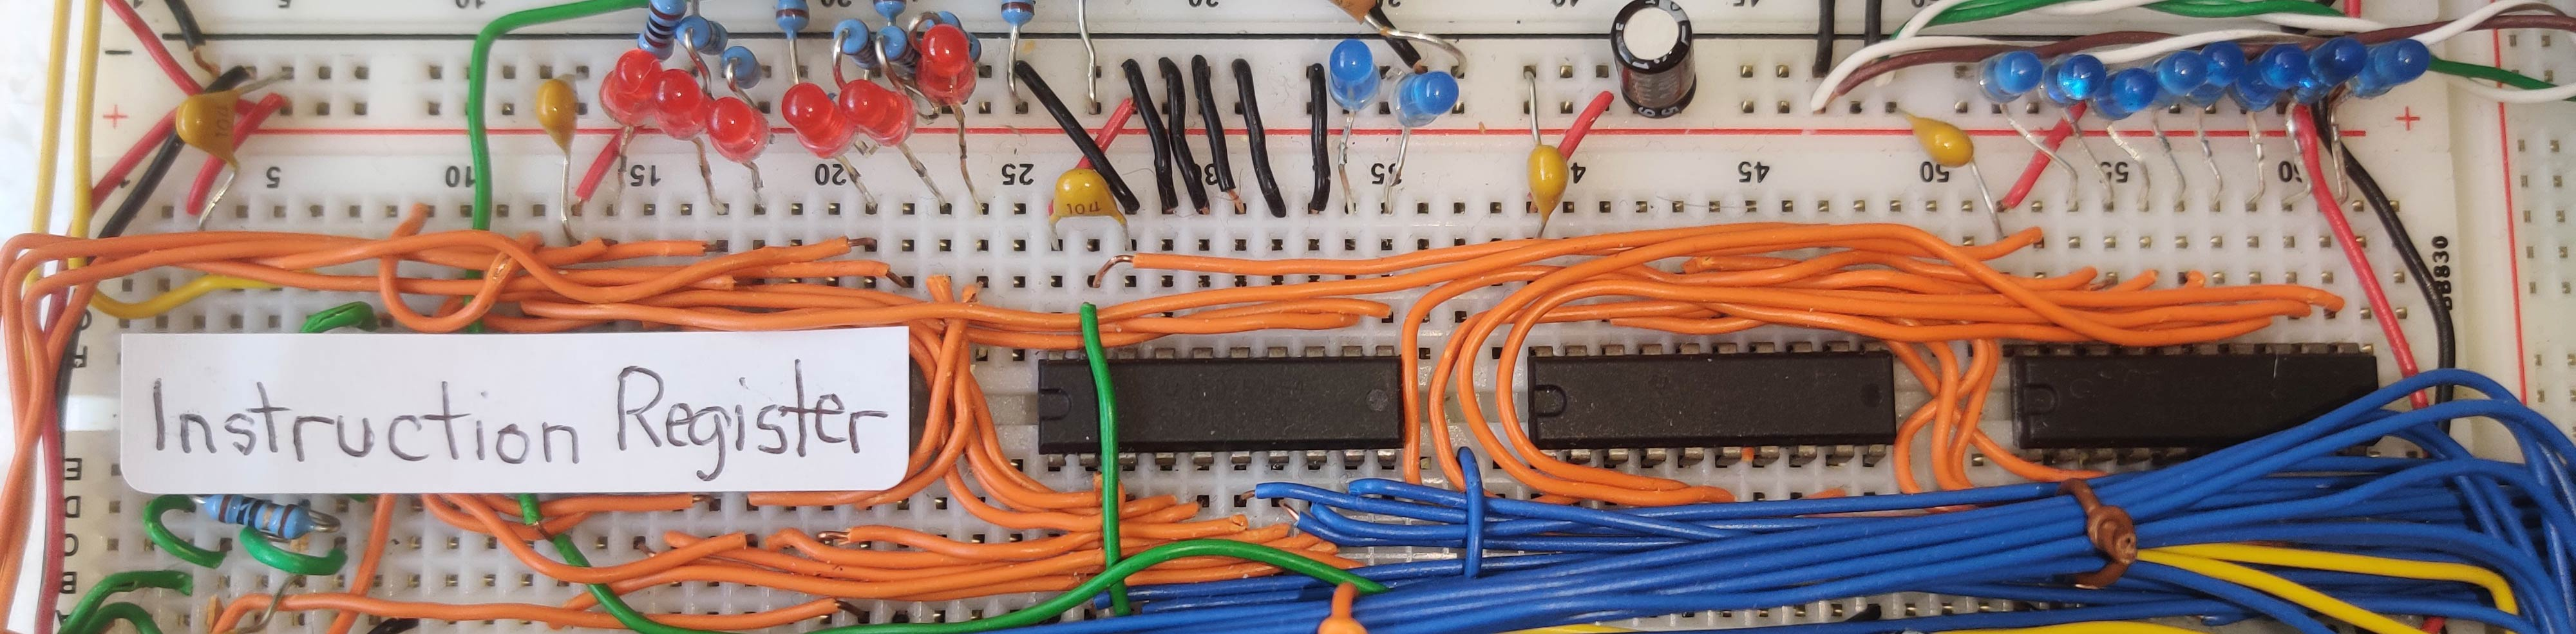
\includegraphics[scale=0.1]{comp/ir}
    \caption{Instruction register implementation}
    \label{ir-i}
  \end{figure}

  \begin{figure}[h]
    \centering
    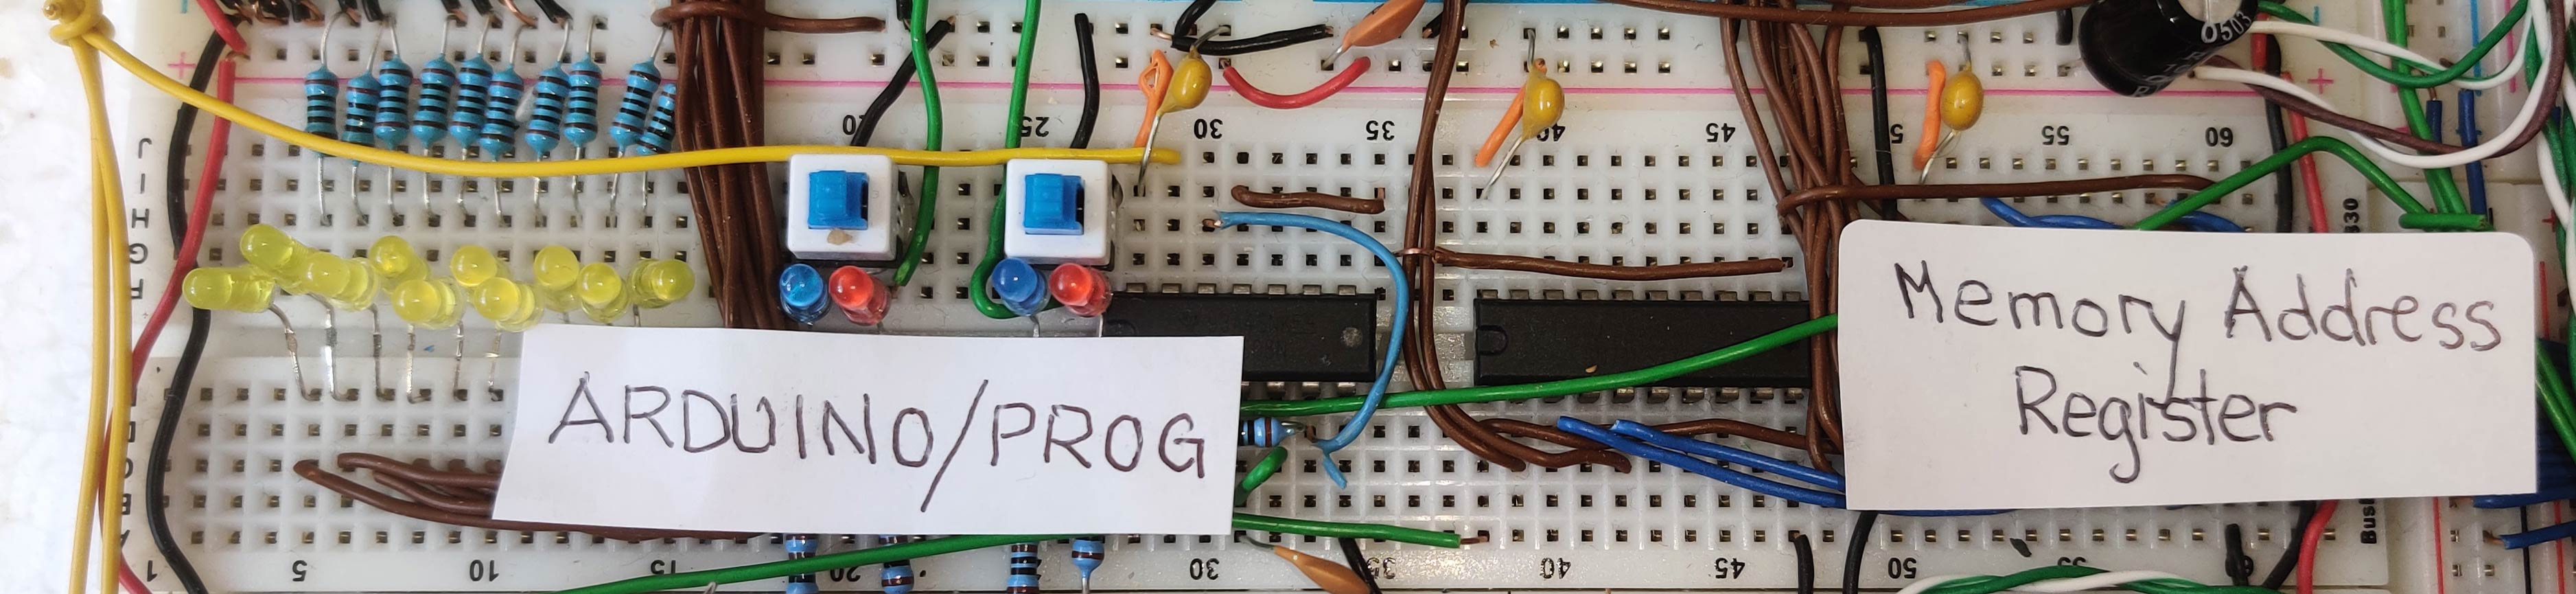
\includegraphics[scale=0.1]{comp/mar}
    \caption{Memory address register implementation}
    \label{mar-i}
  \end{figure}

  \begin{figure}[h]
    \centering
    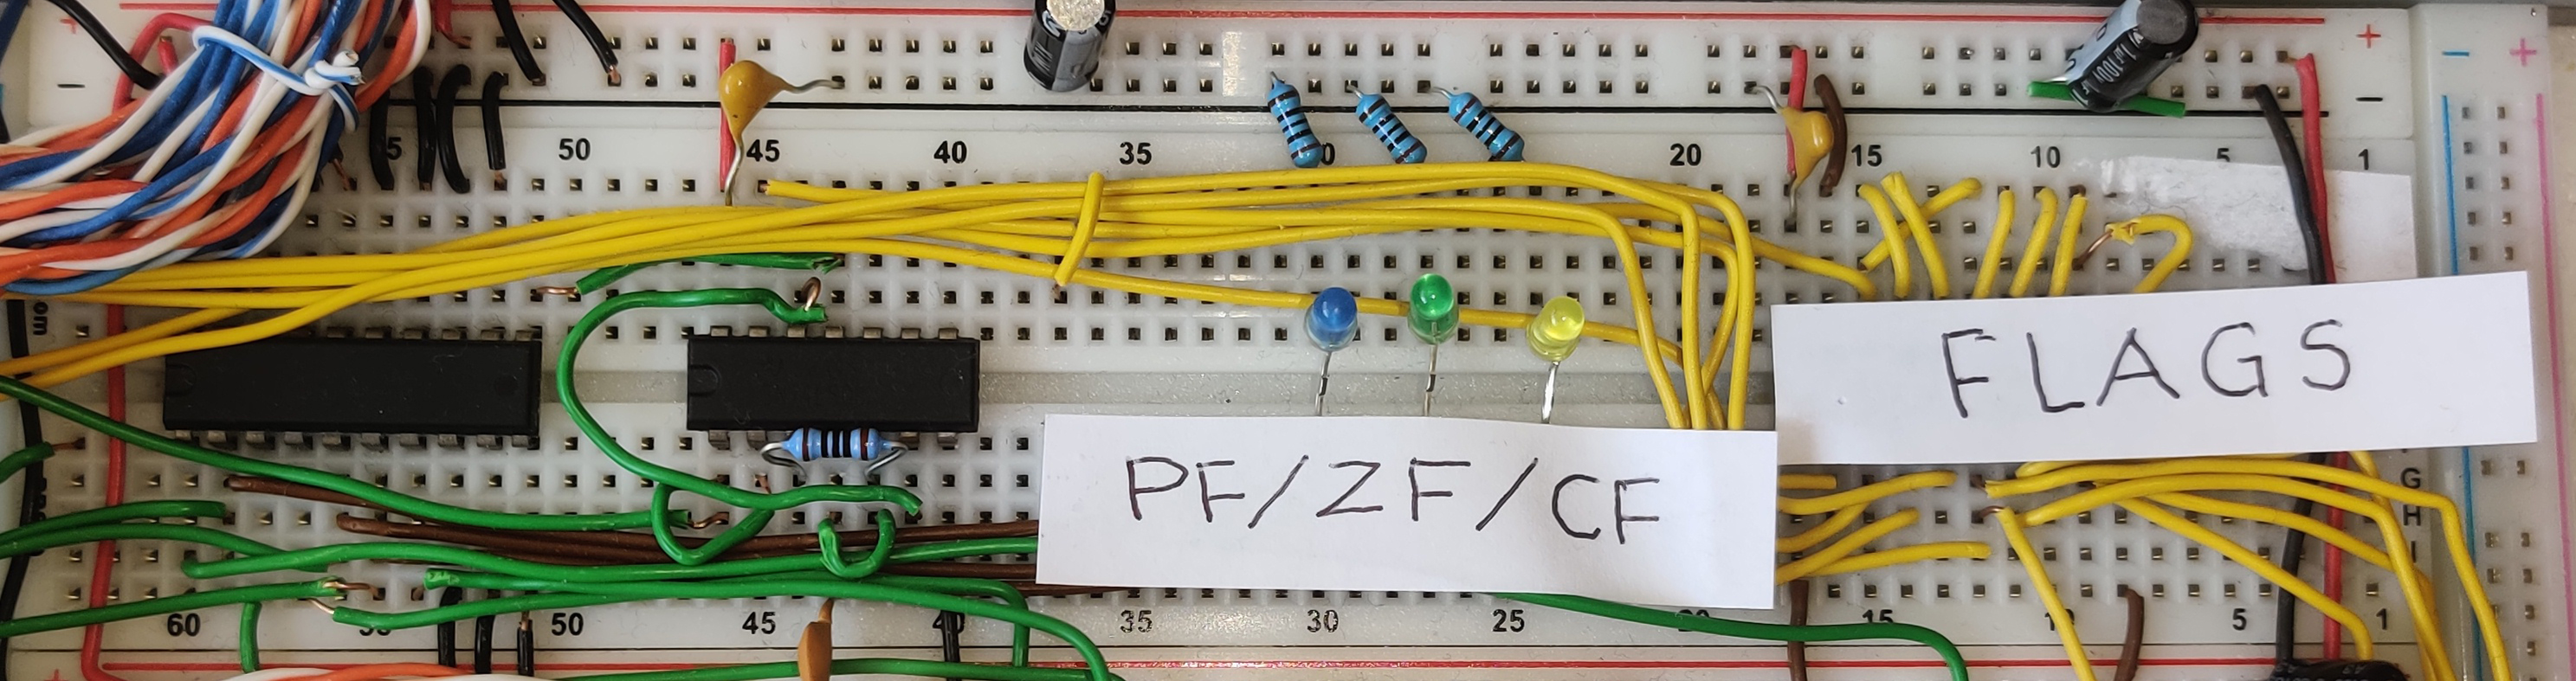
\includegraphics[scale=0.1]{comp/flags}
    \caption{Flags register implementation}
    \label{flags-i}
  \end{figure}

  \begin{figure}[h]
    \centering
    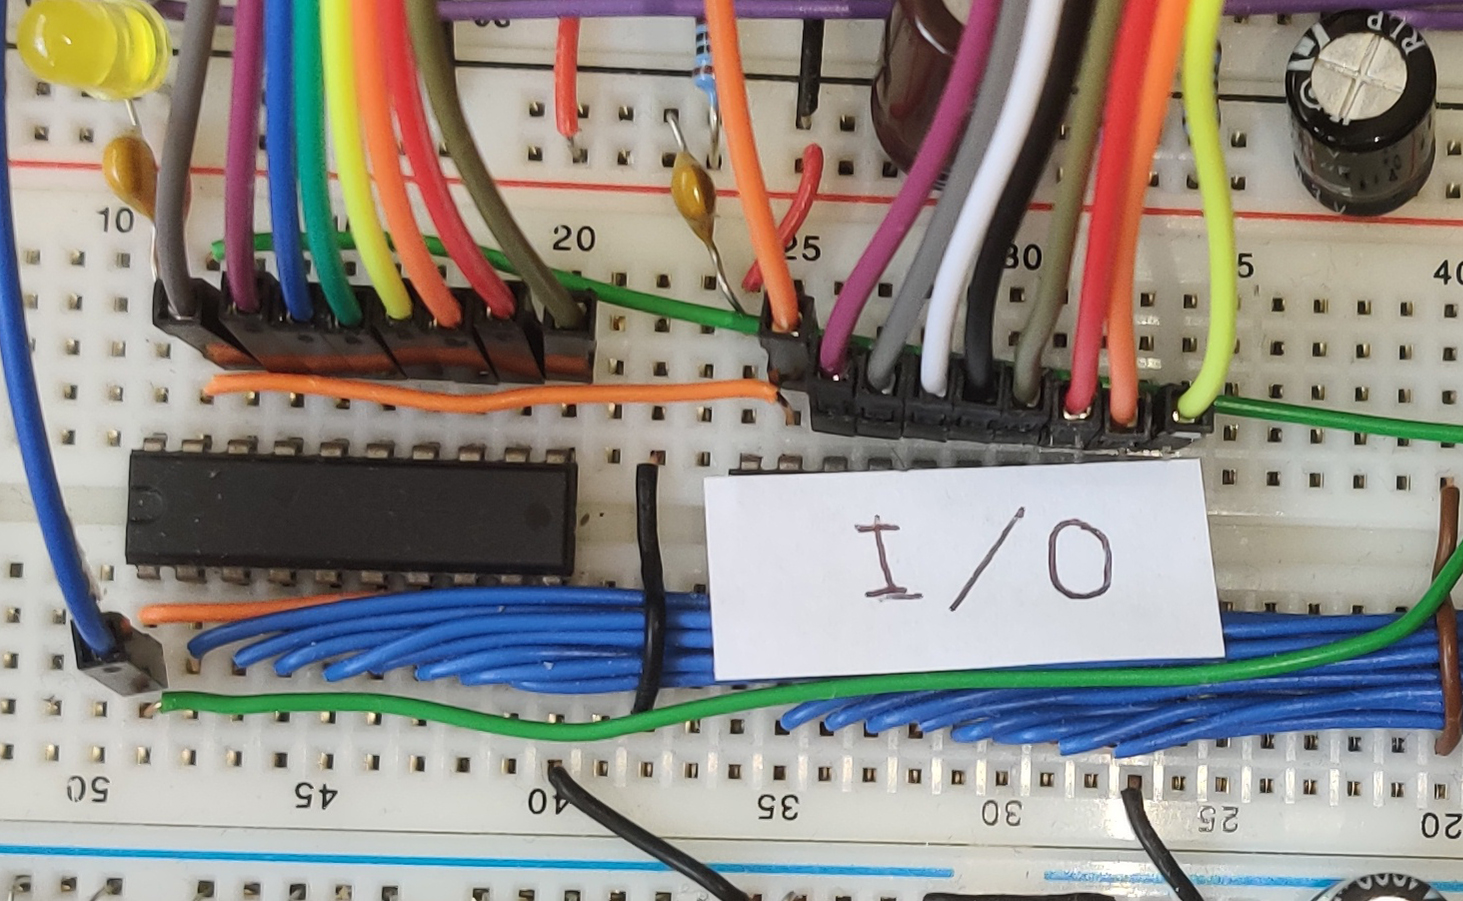
\includegraphics[scale=0.1]{comp/io}
    \caption{Input/Output implementation}
    \label{io-i}
  \end{figure}

  \begin{figure}[h]
    \centering
    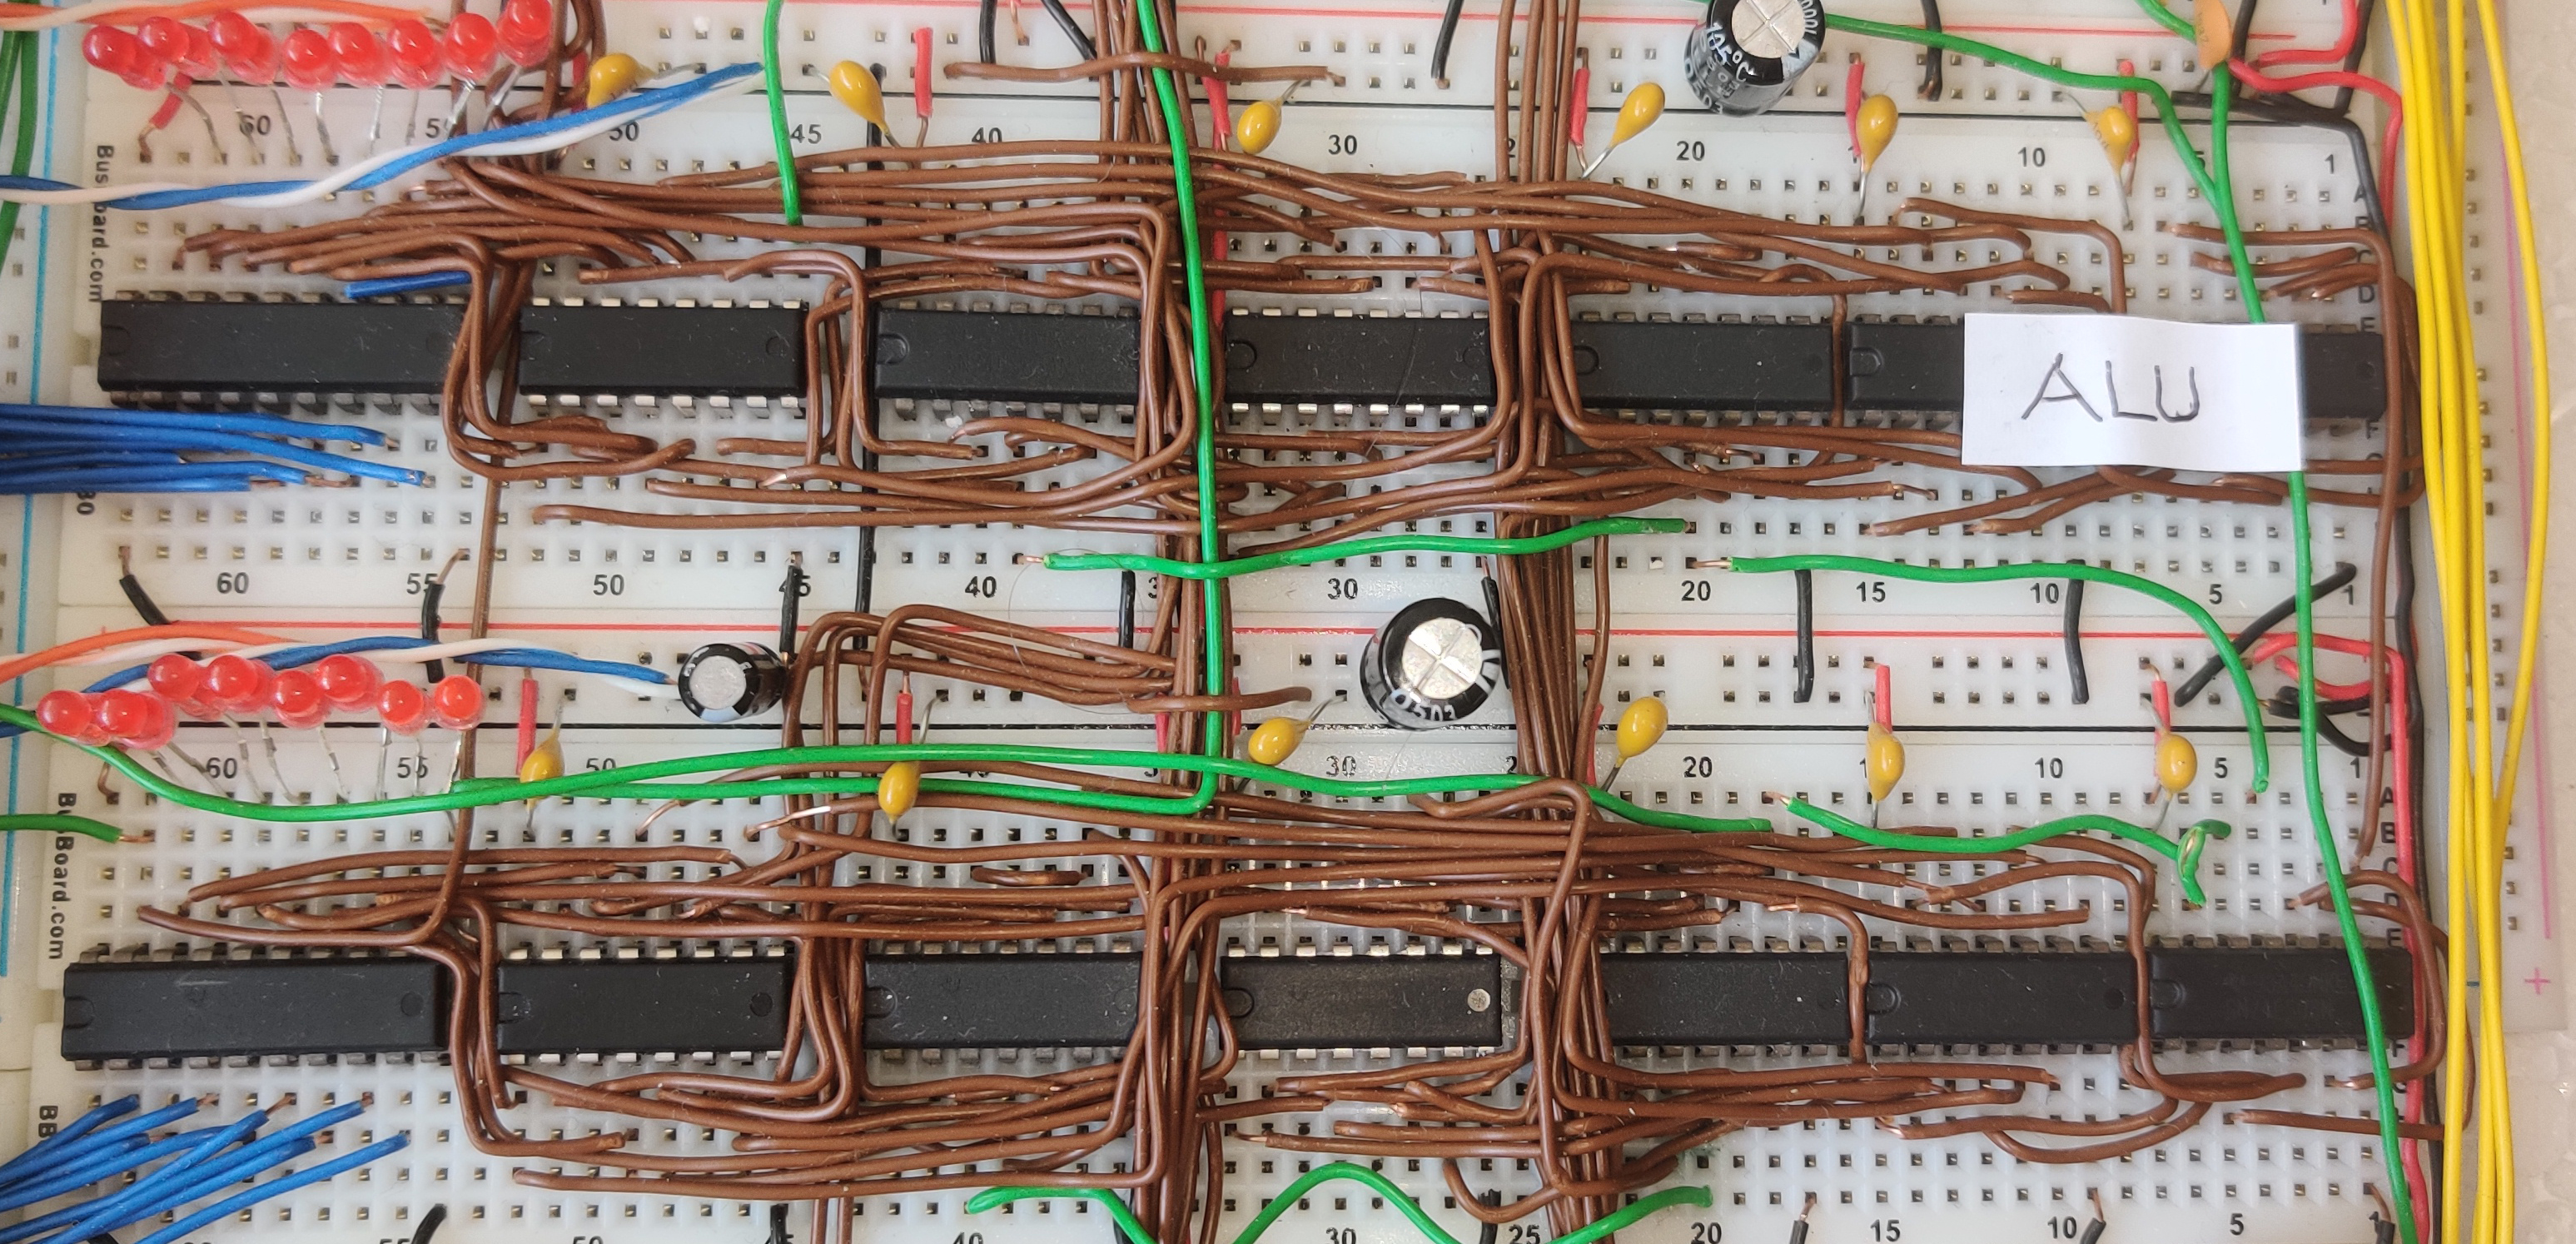
\includegraphics[scale=0.1]{comp/alu}
    \caption{Arithmetic-Logic Unit implementation}
    \label{alu-i}
  \end{figure}

  \begin{figure}[h]
    \centering
    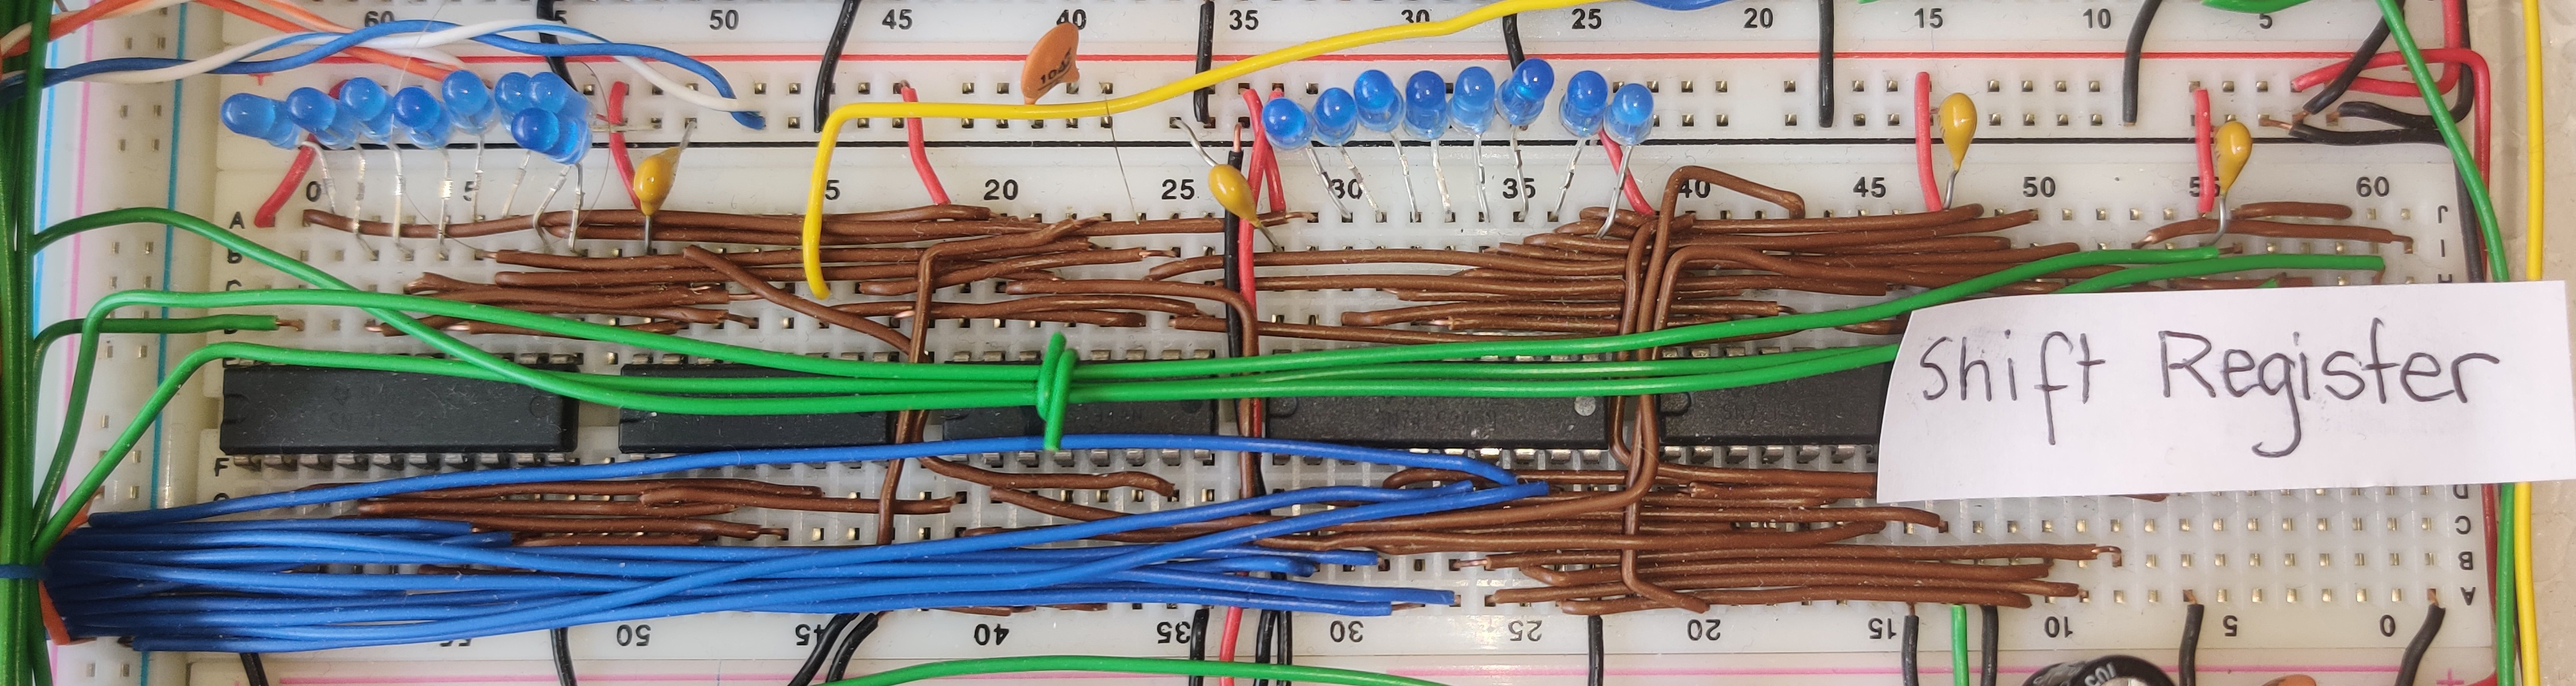
\includegraphics[scale=0.1]{comp/shift-reg}
    \caption{Shift Register implementation}
    \label{shift-reg-i}
  \end{figure}

  \begin{figure}[h]
    \centering
    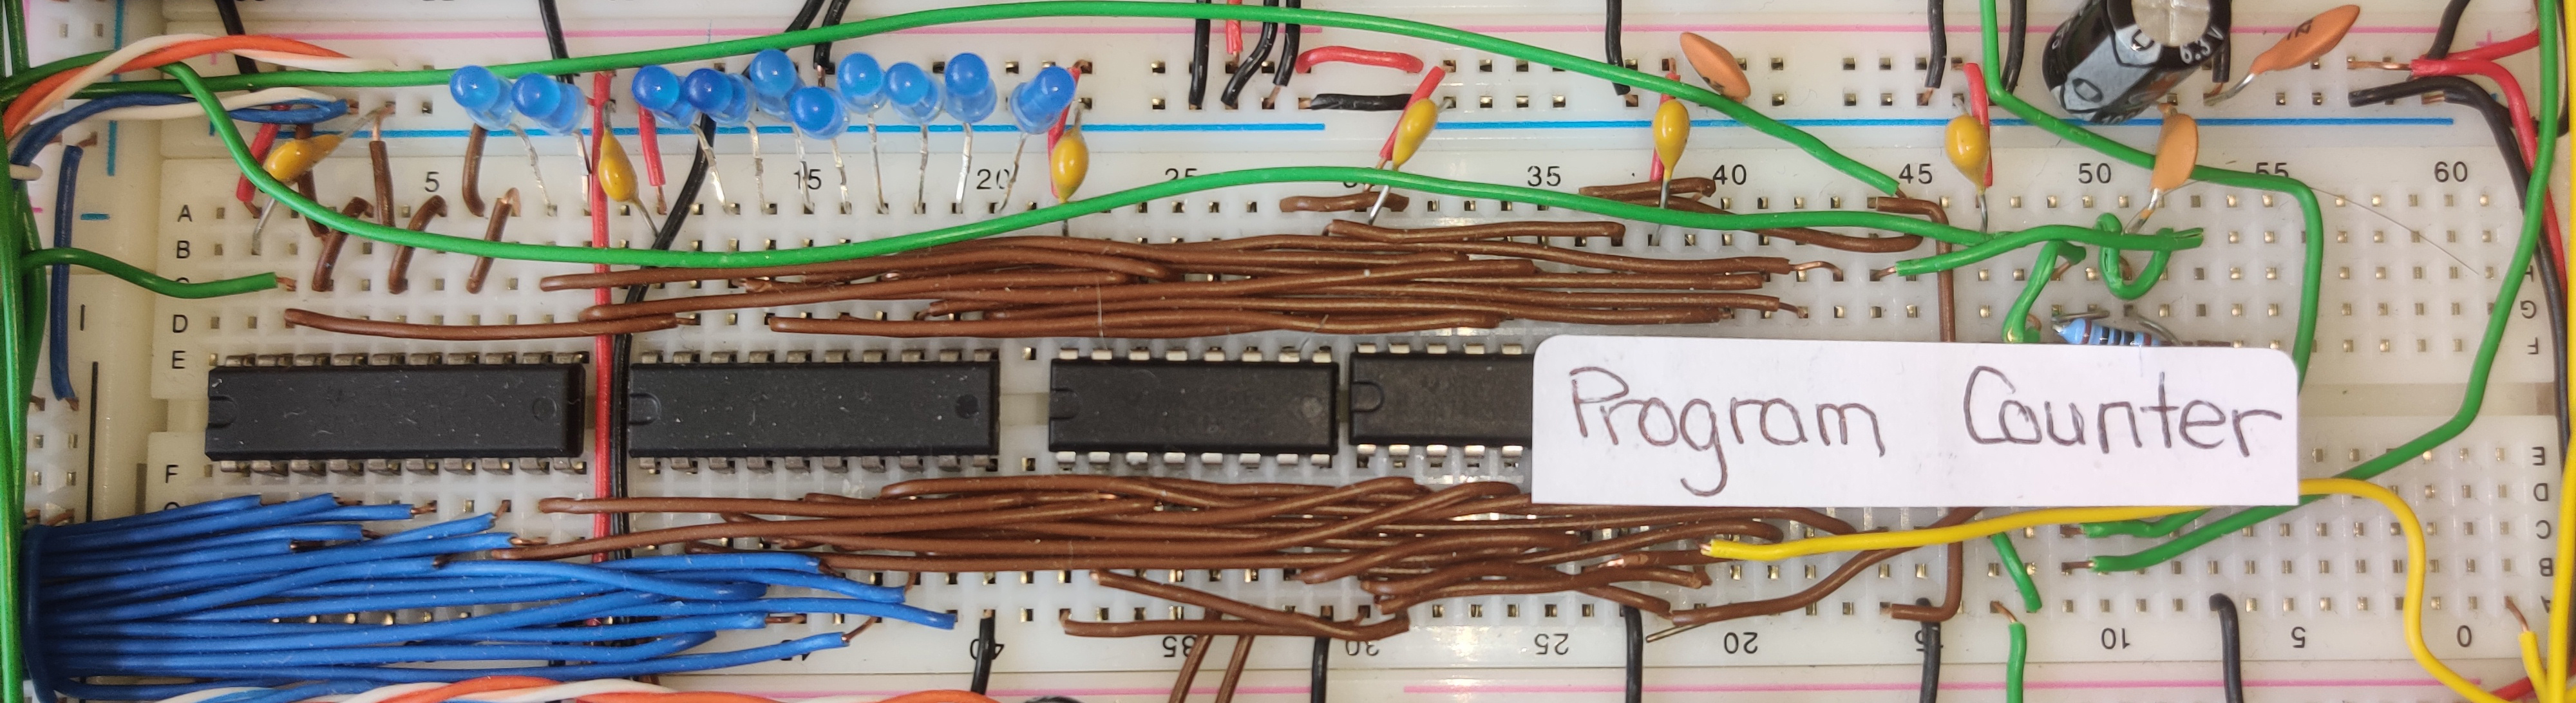
\includegraphics[scale=0.1]{comp/pc}
    \caption{Program Counter implementation}
    \label{pc-i}
  \end{figure}

  \begin{figure}[h]
    \centering
    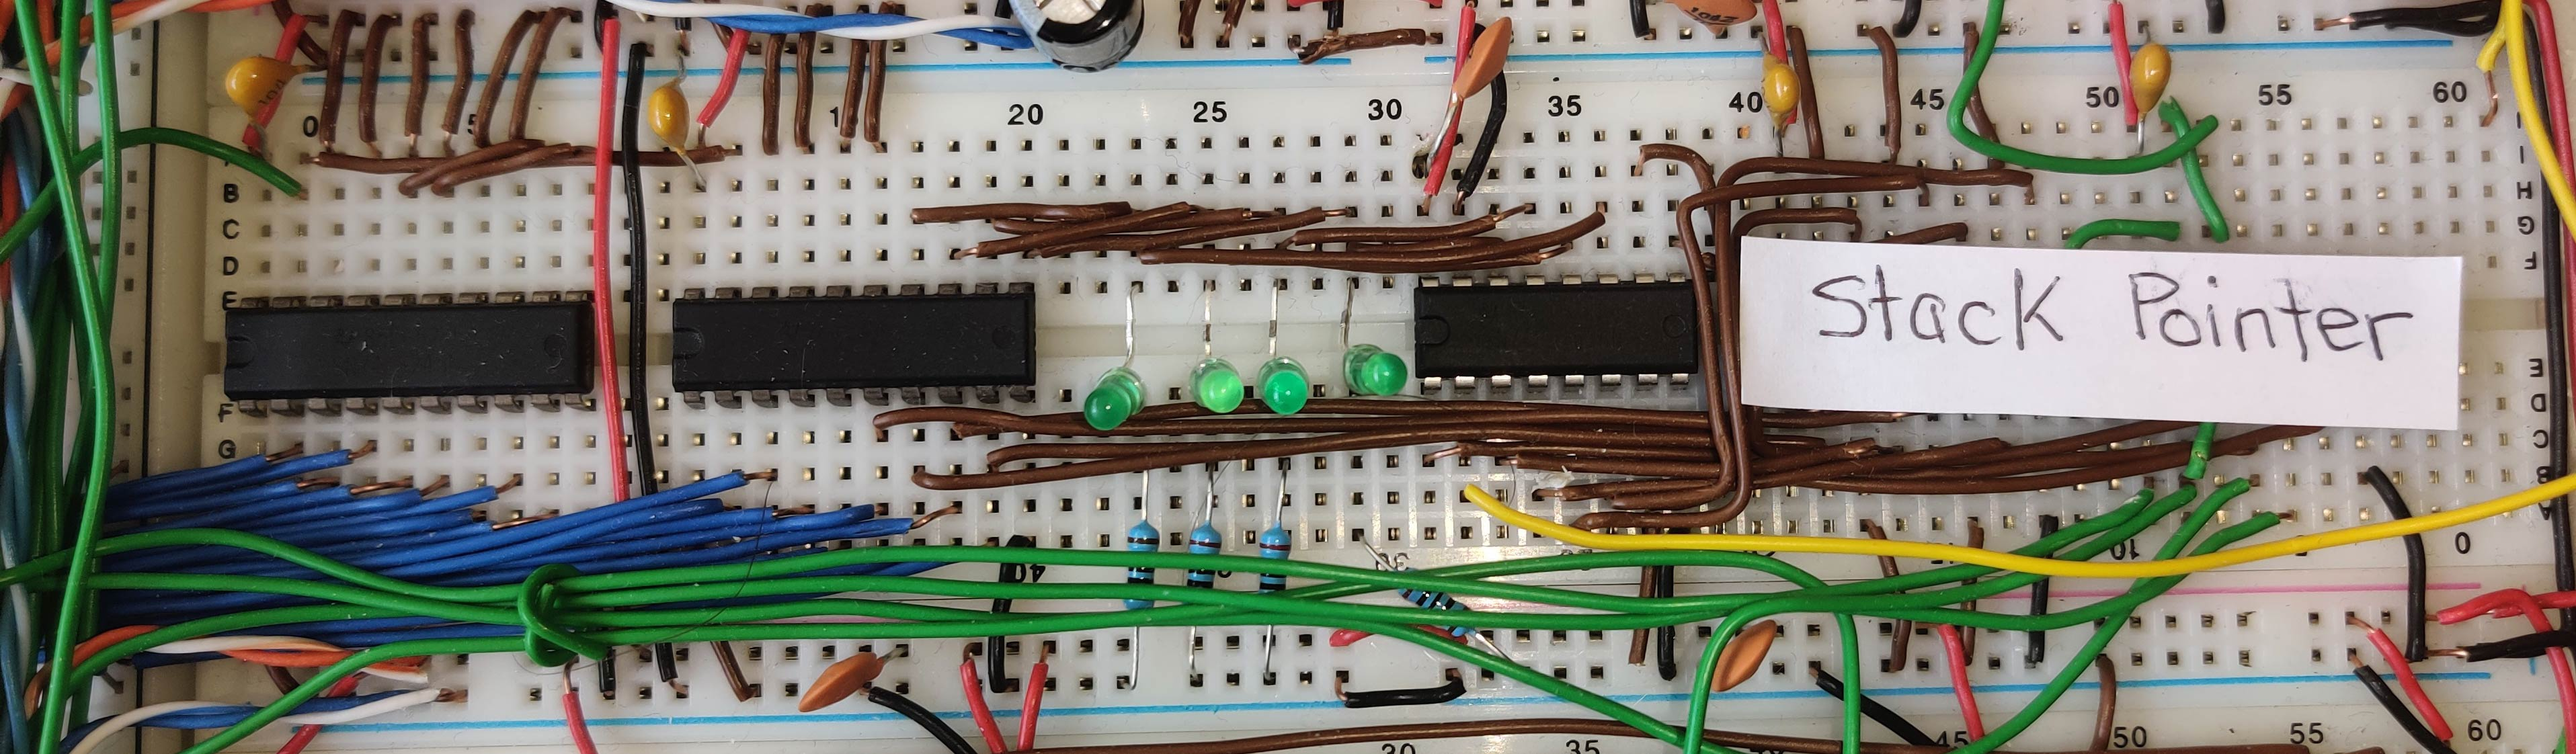
\includegraphics[scale=0.1]{comp/sp}
    \caption{Stack Pointer implementation}
    \label{sp-i}
  \end{figure}

  \begin{figure}[h]
    \centering
    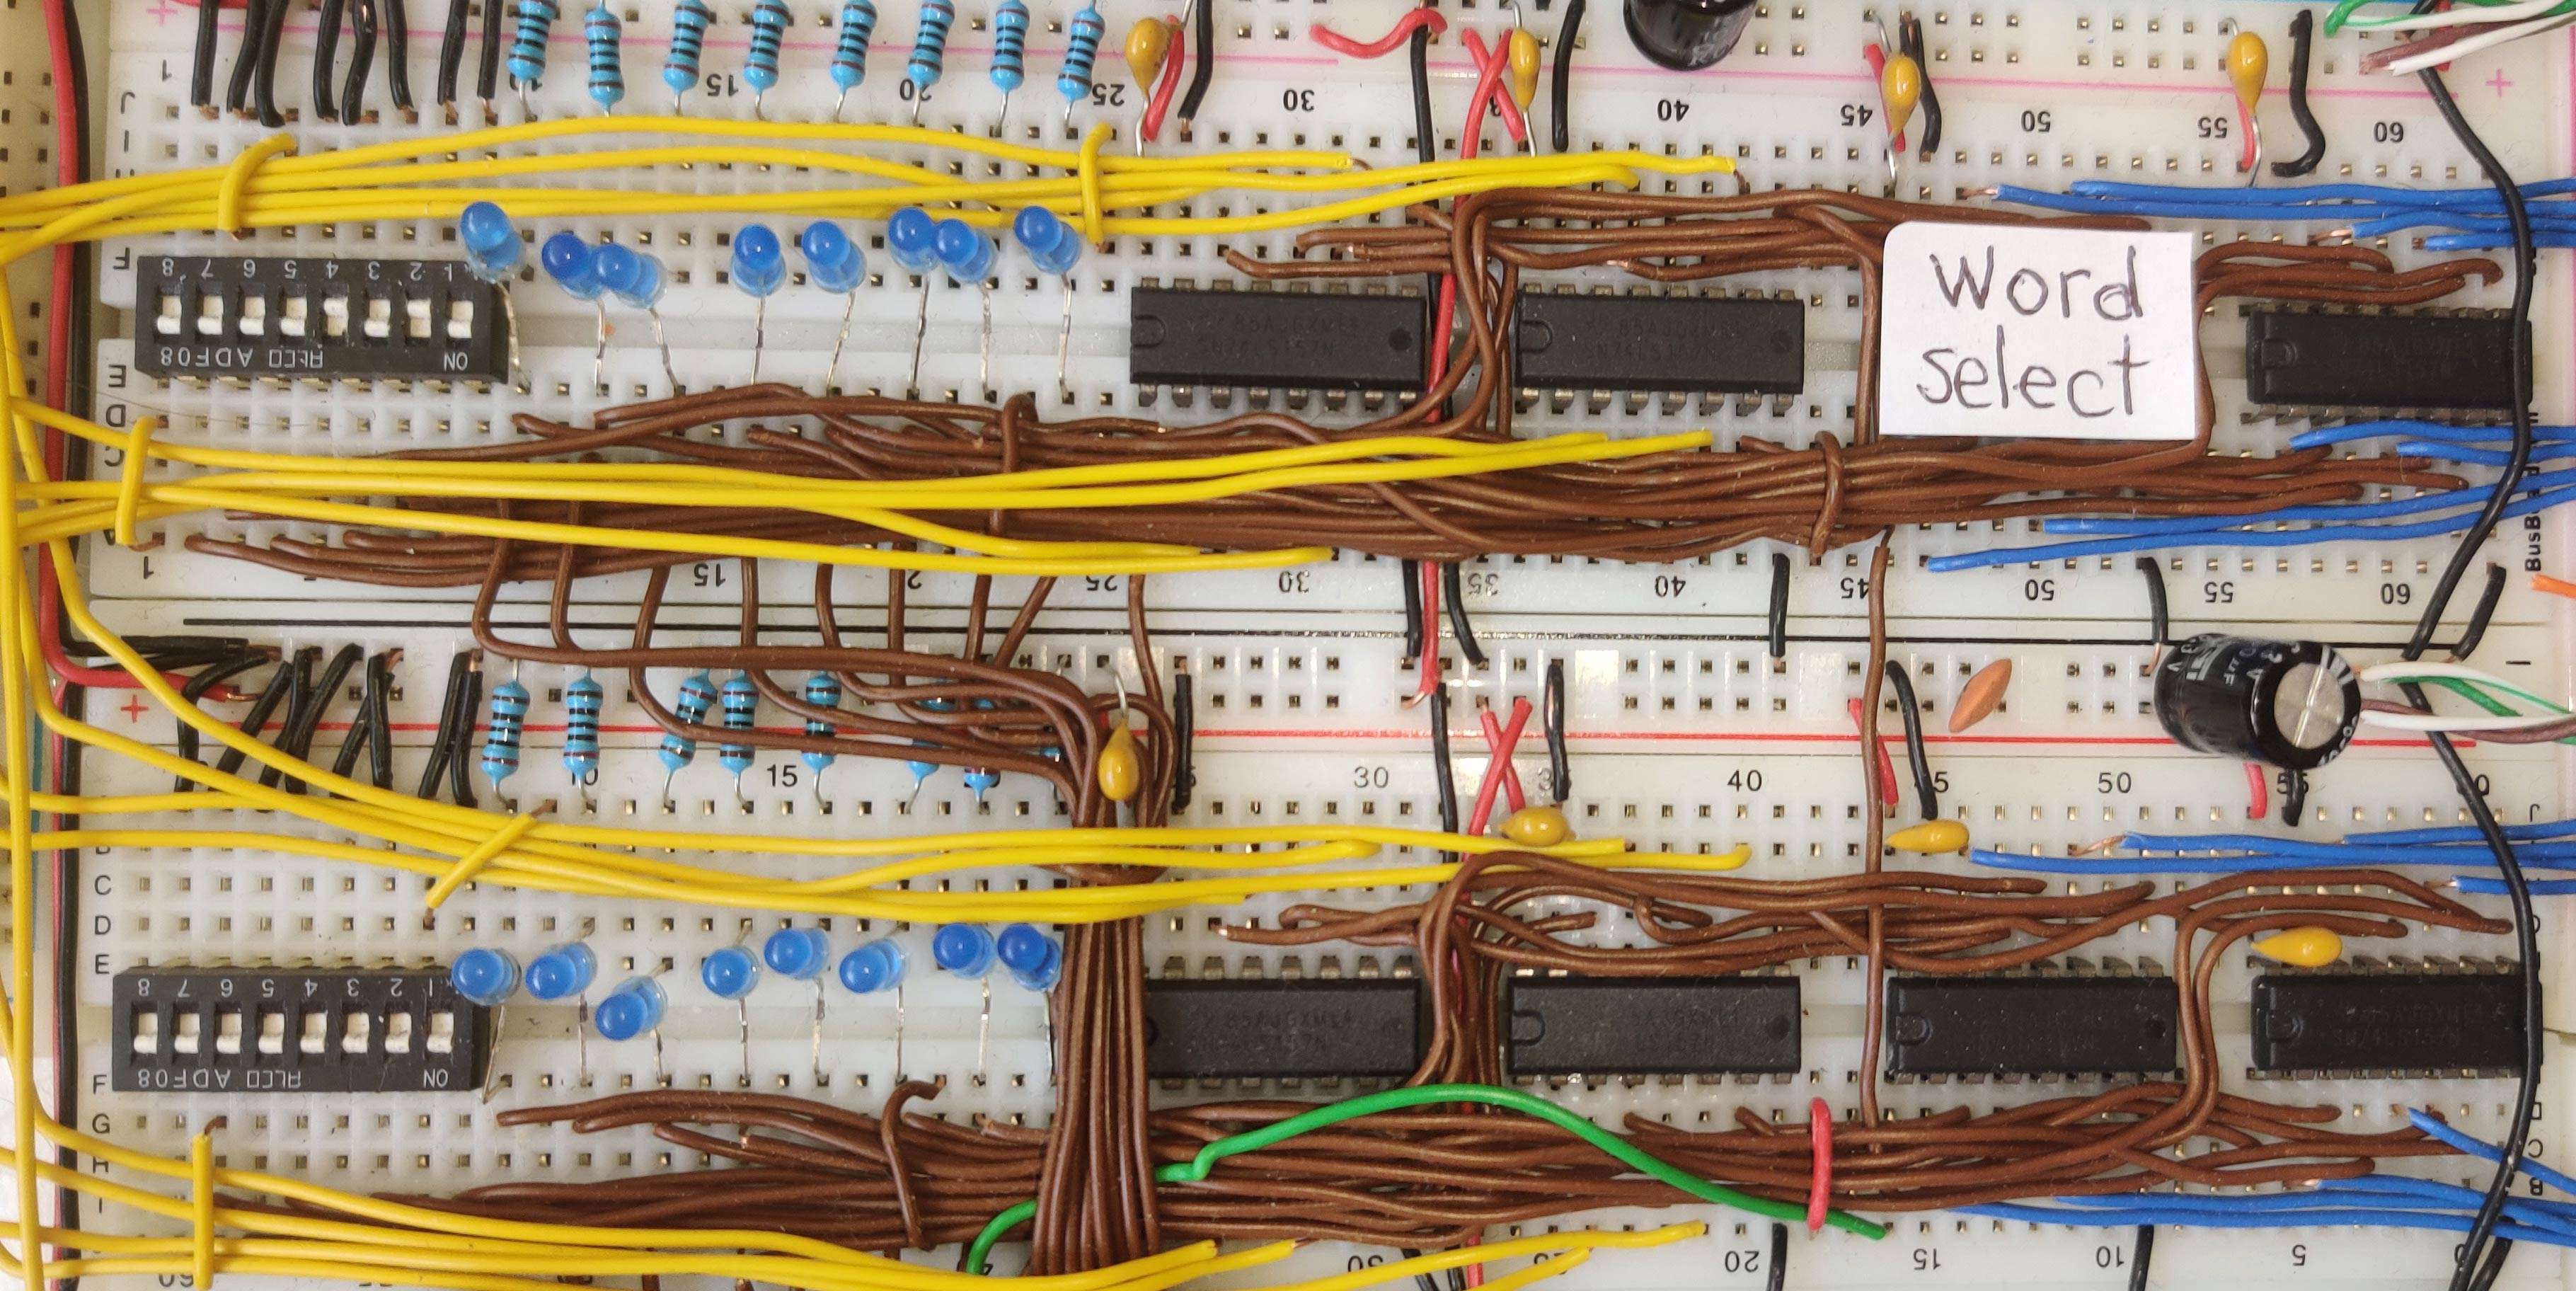
\includegraphics[scale=0.1]{comp/word-select}
    \caption{Word selector implementation}
    \label{word-select-i}
  \end{figure}

  \begin{figure}[h]
    \centering
    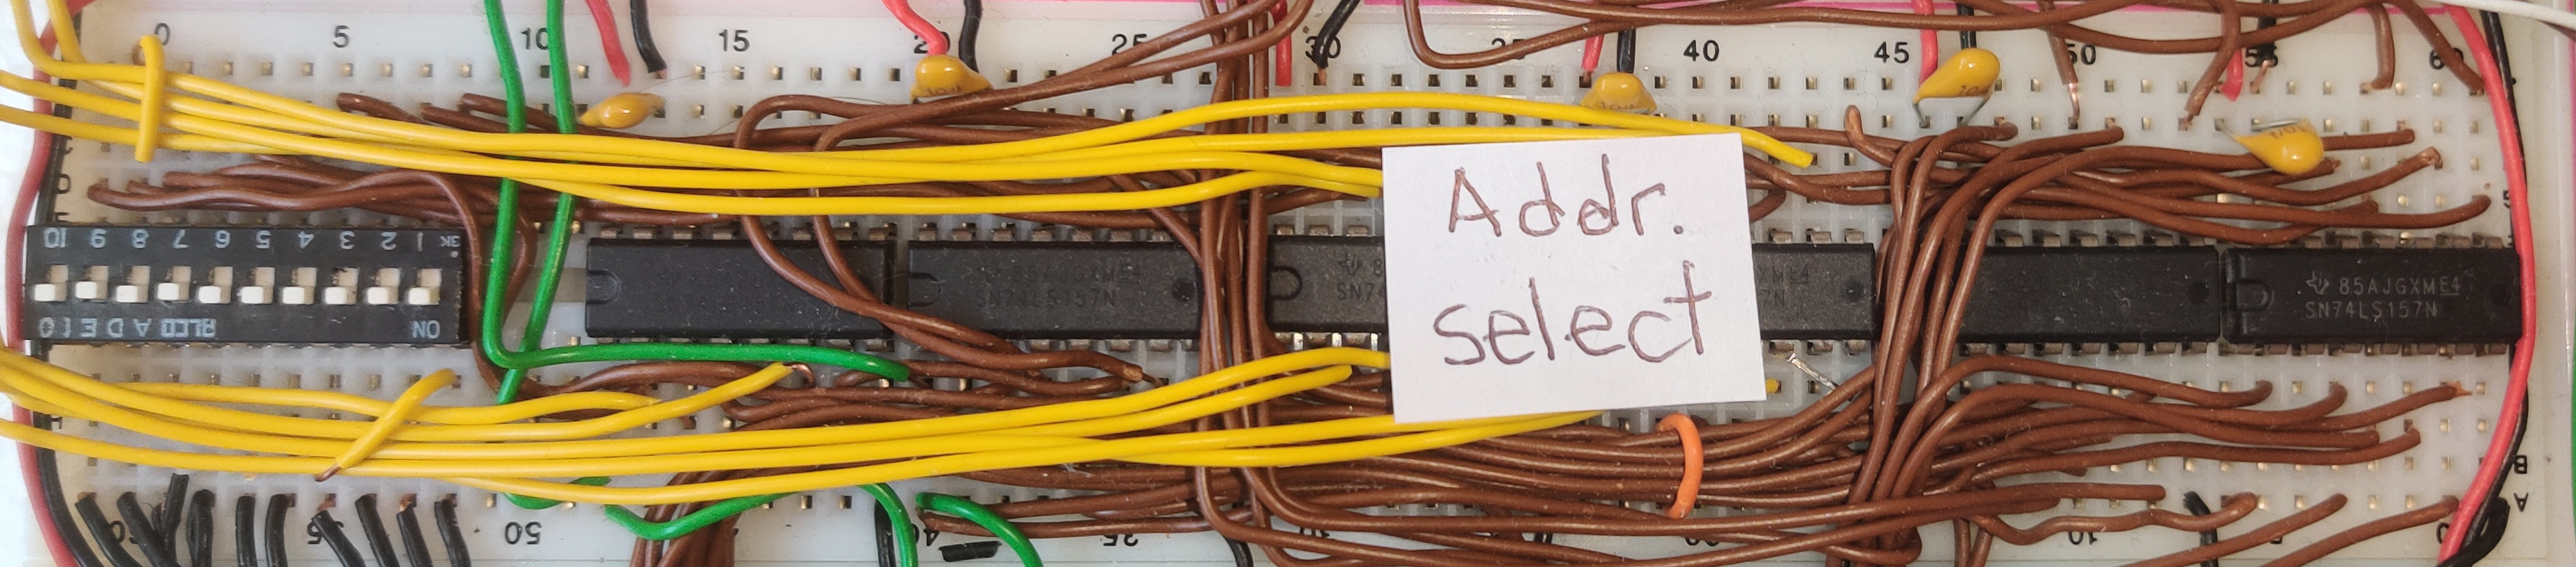
\includegraphics[scale=0.1]{comp/addr-select}
    \caption{Address selector implementation}
    \label{addr-select-i}
  \end{figure}

  \begin{figure}[h]
    \centering
    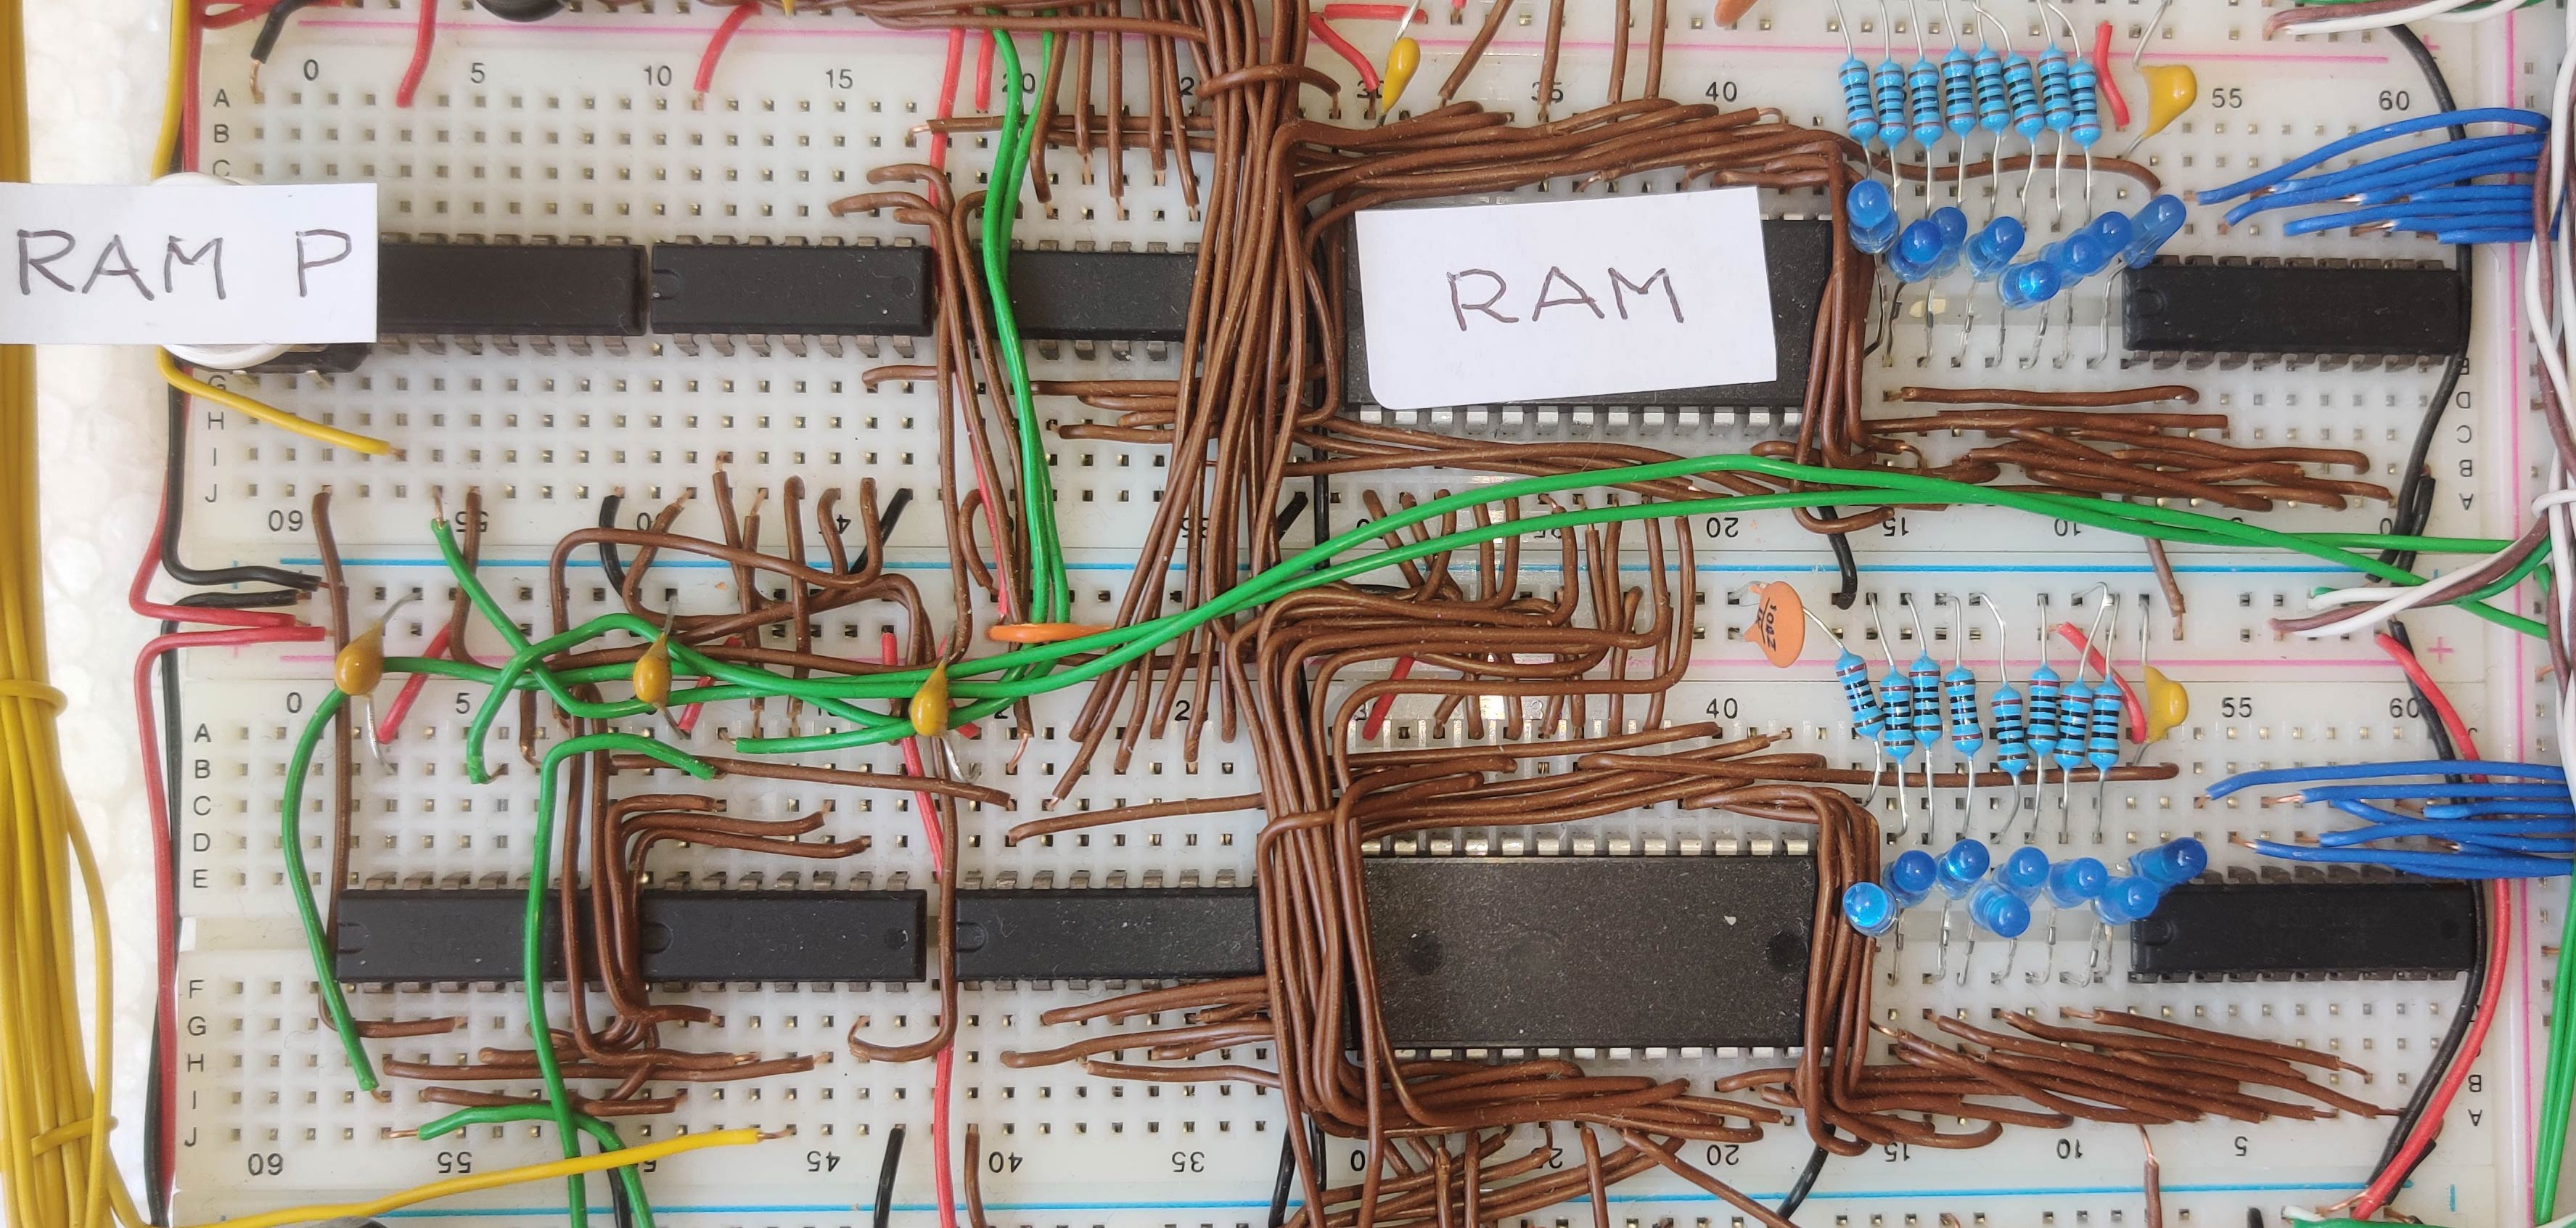
\includegraphics[scale=0.1]{comp/ram}
    \caption{Random Access Memory implementation}
    \label{ram-i}
  \end{figure}

  \begin{figure}[h]
    \centering
    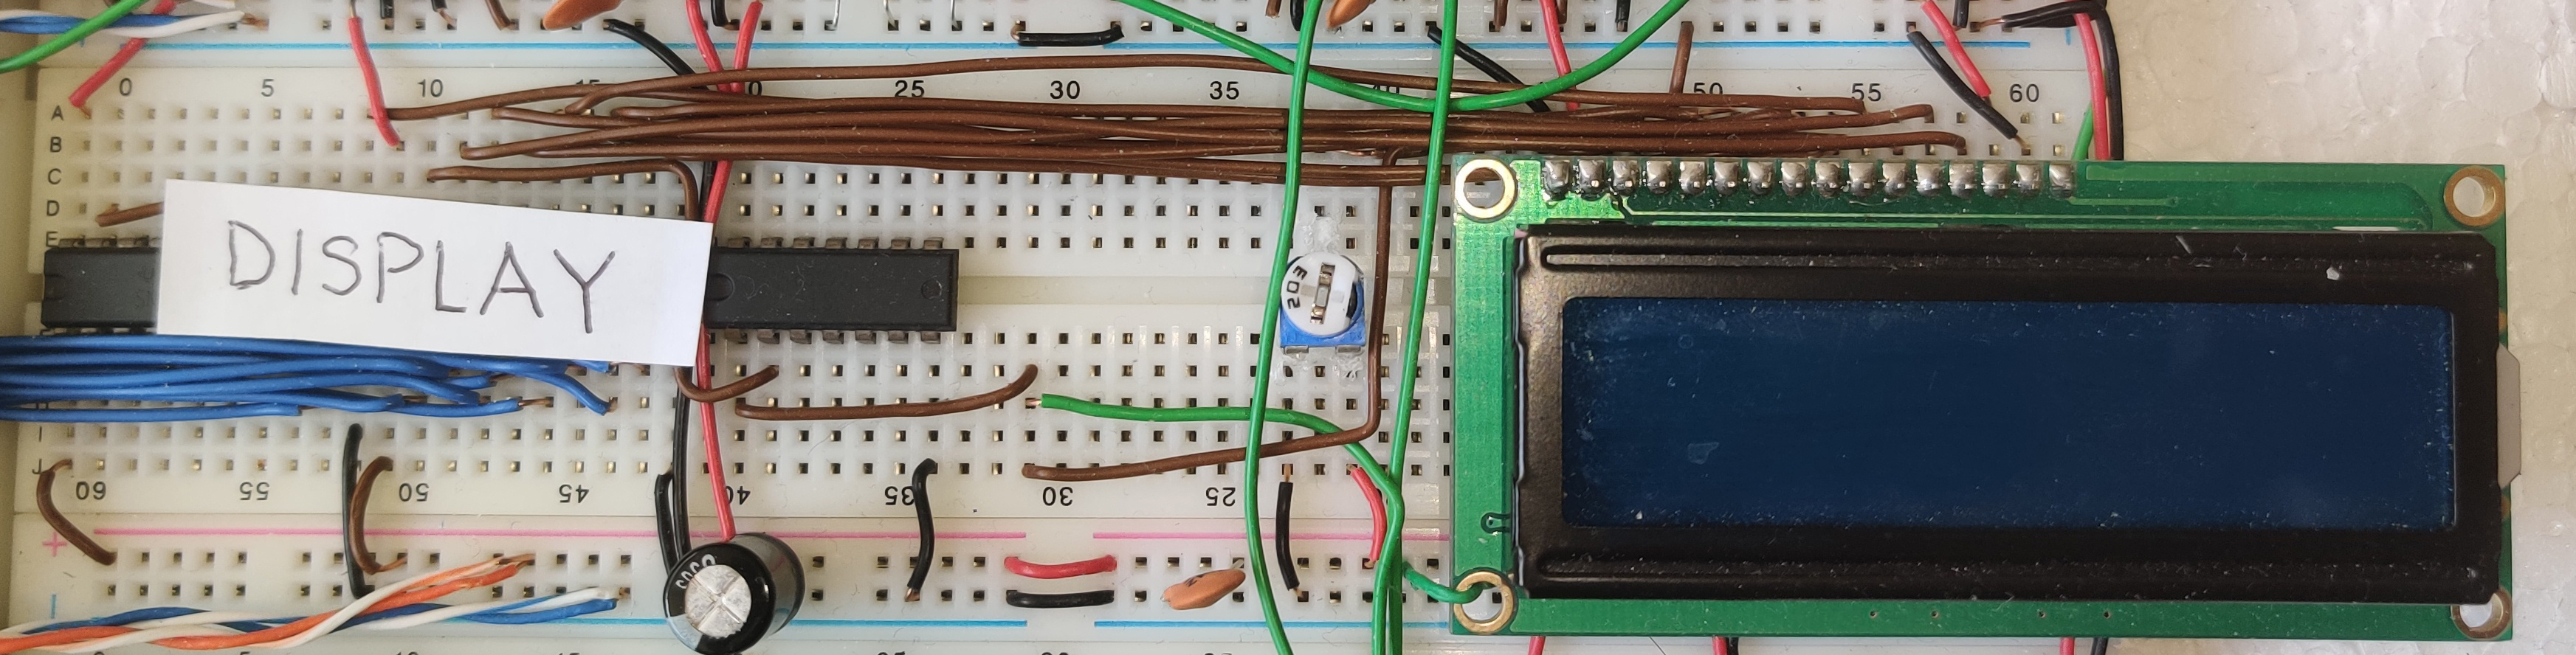
\includegraphics[scale=0.1]{comp/display}
    \caption{Display implementation}
    \label{display-i}
  \end{figure}

  \begin{figure}[h]
    \centering
    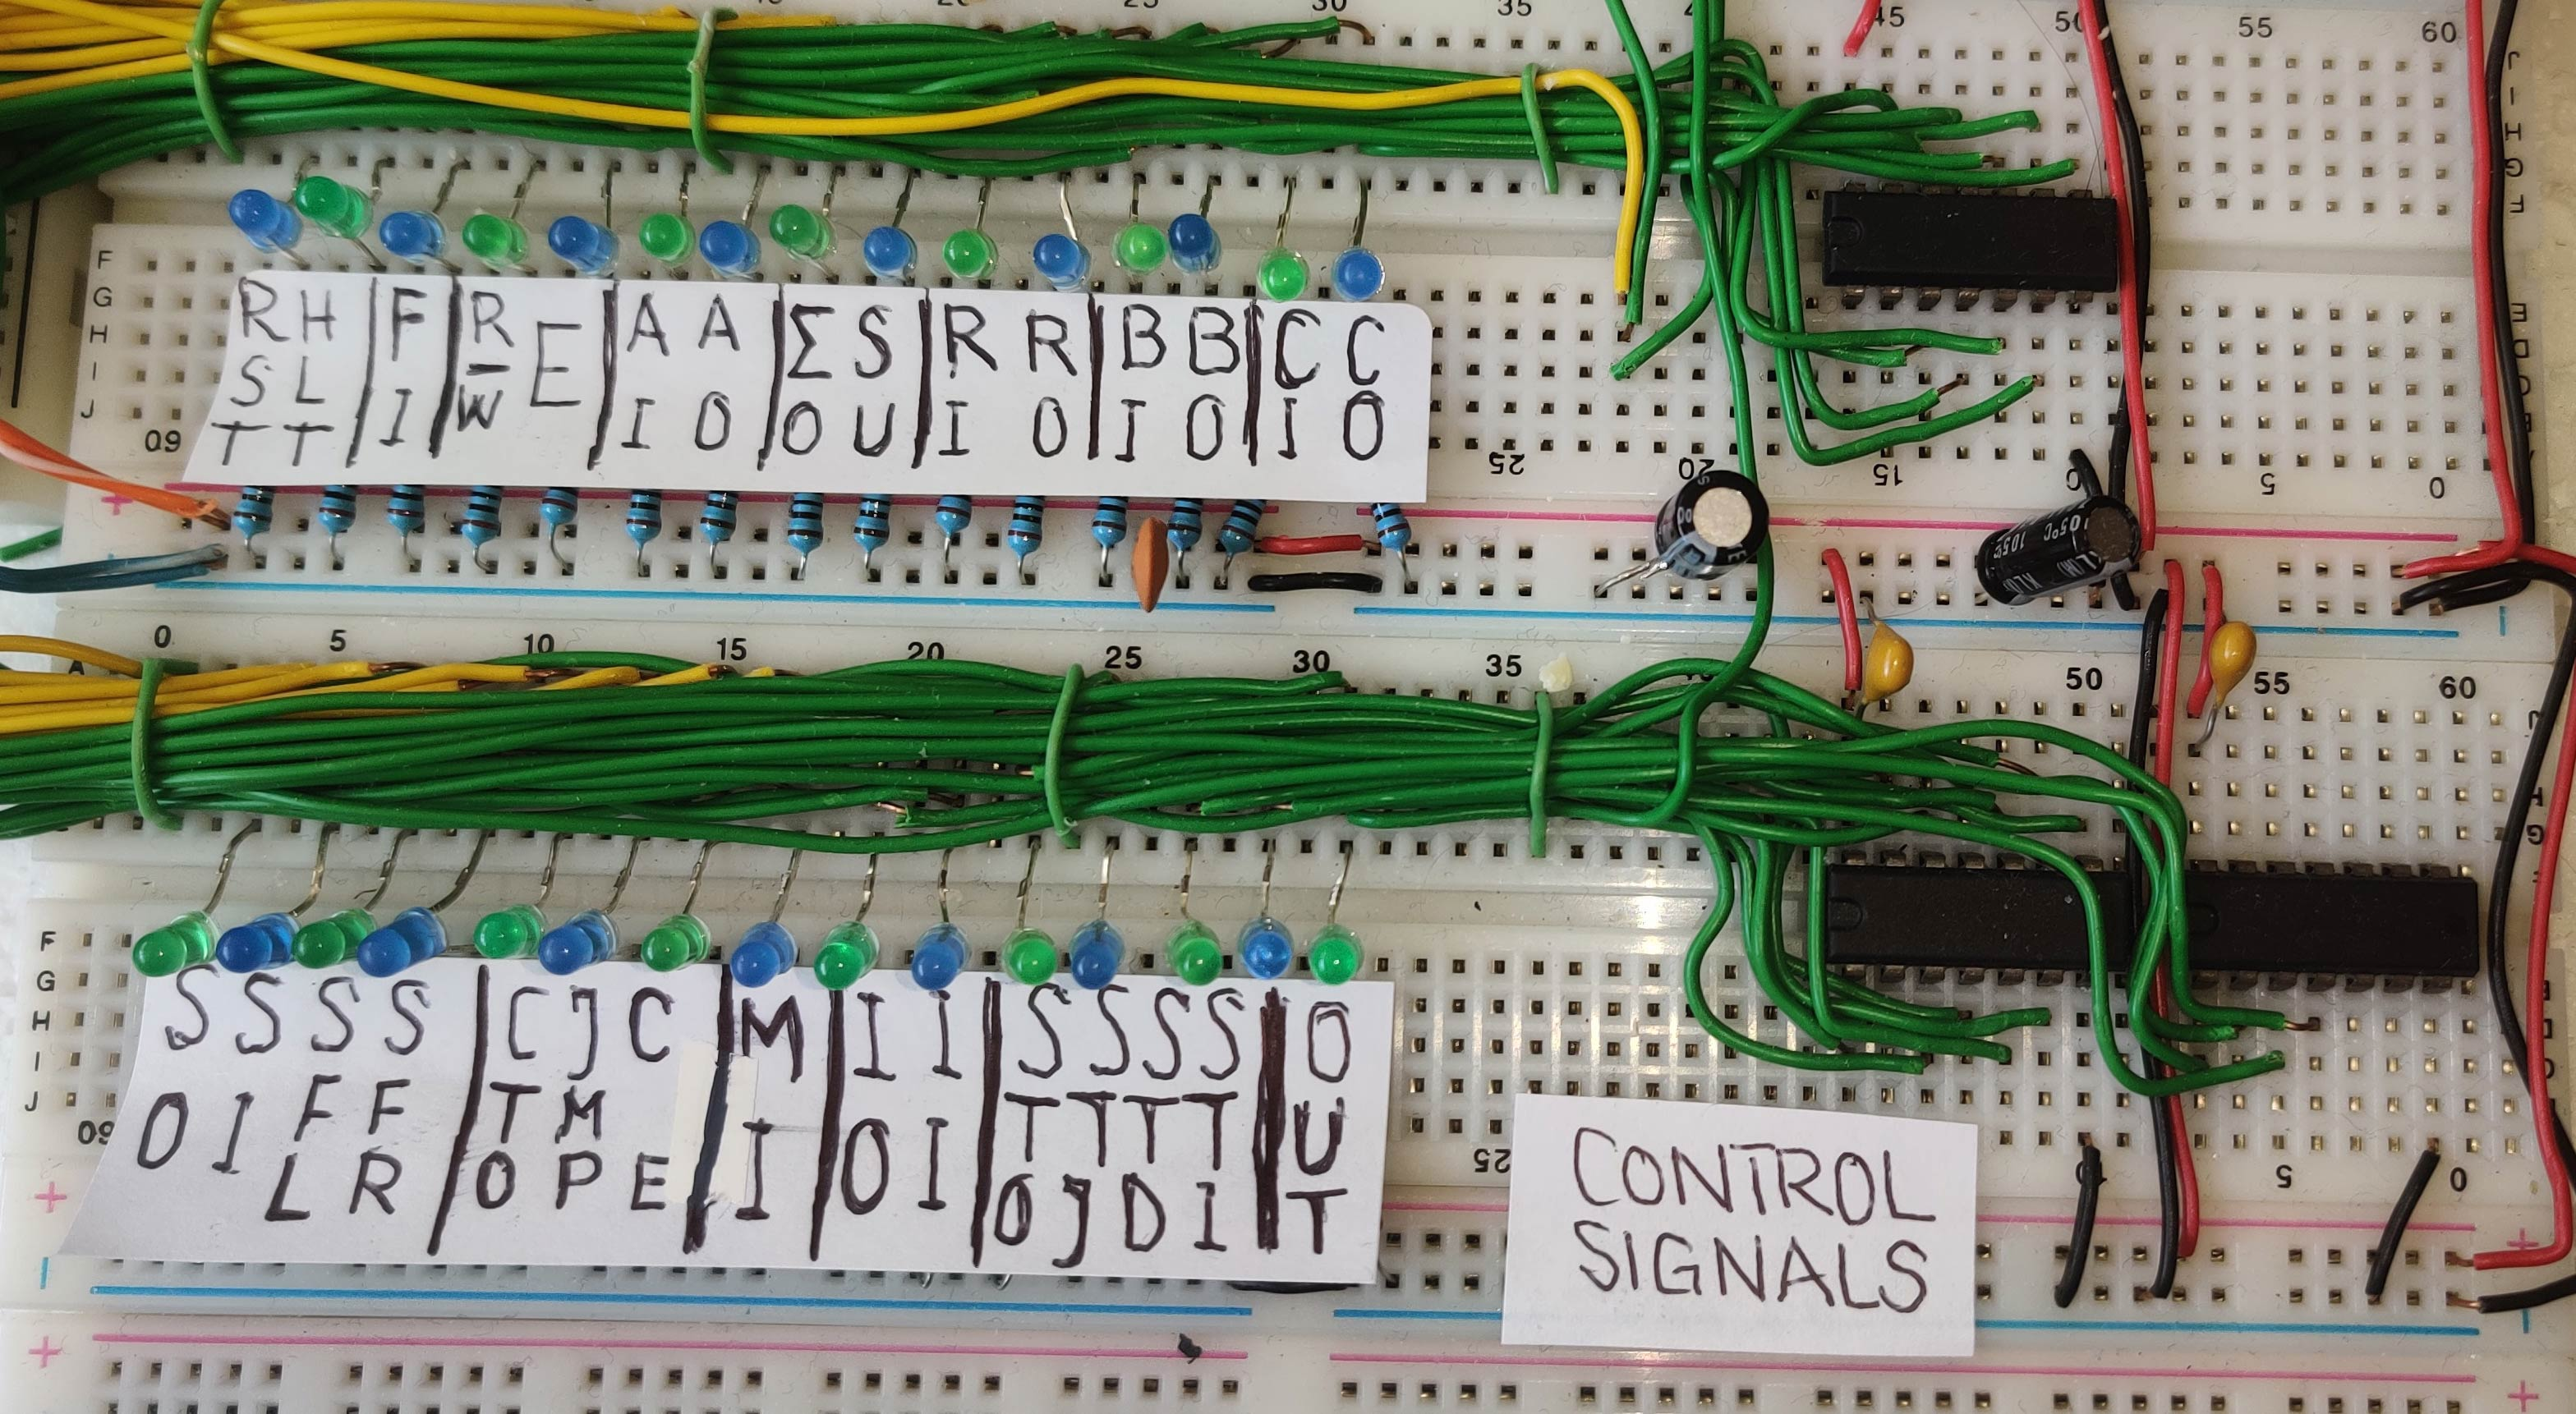
\includegraphics[scale=0.1]{comp/control-sigs}
    \caption{Implementation of the contol signals module}
    \label{control-sigs-i}
  \end{figure}

  \begin{figure}[h]
    \centering
    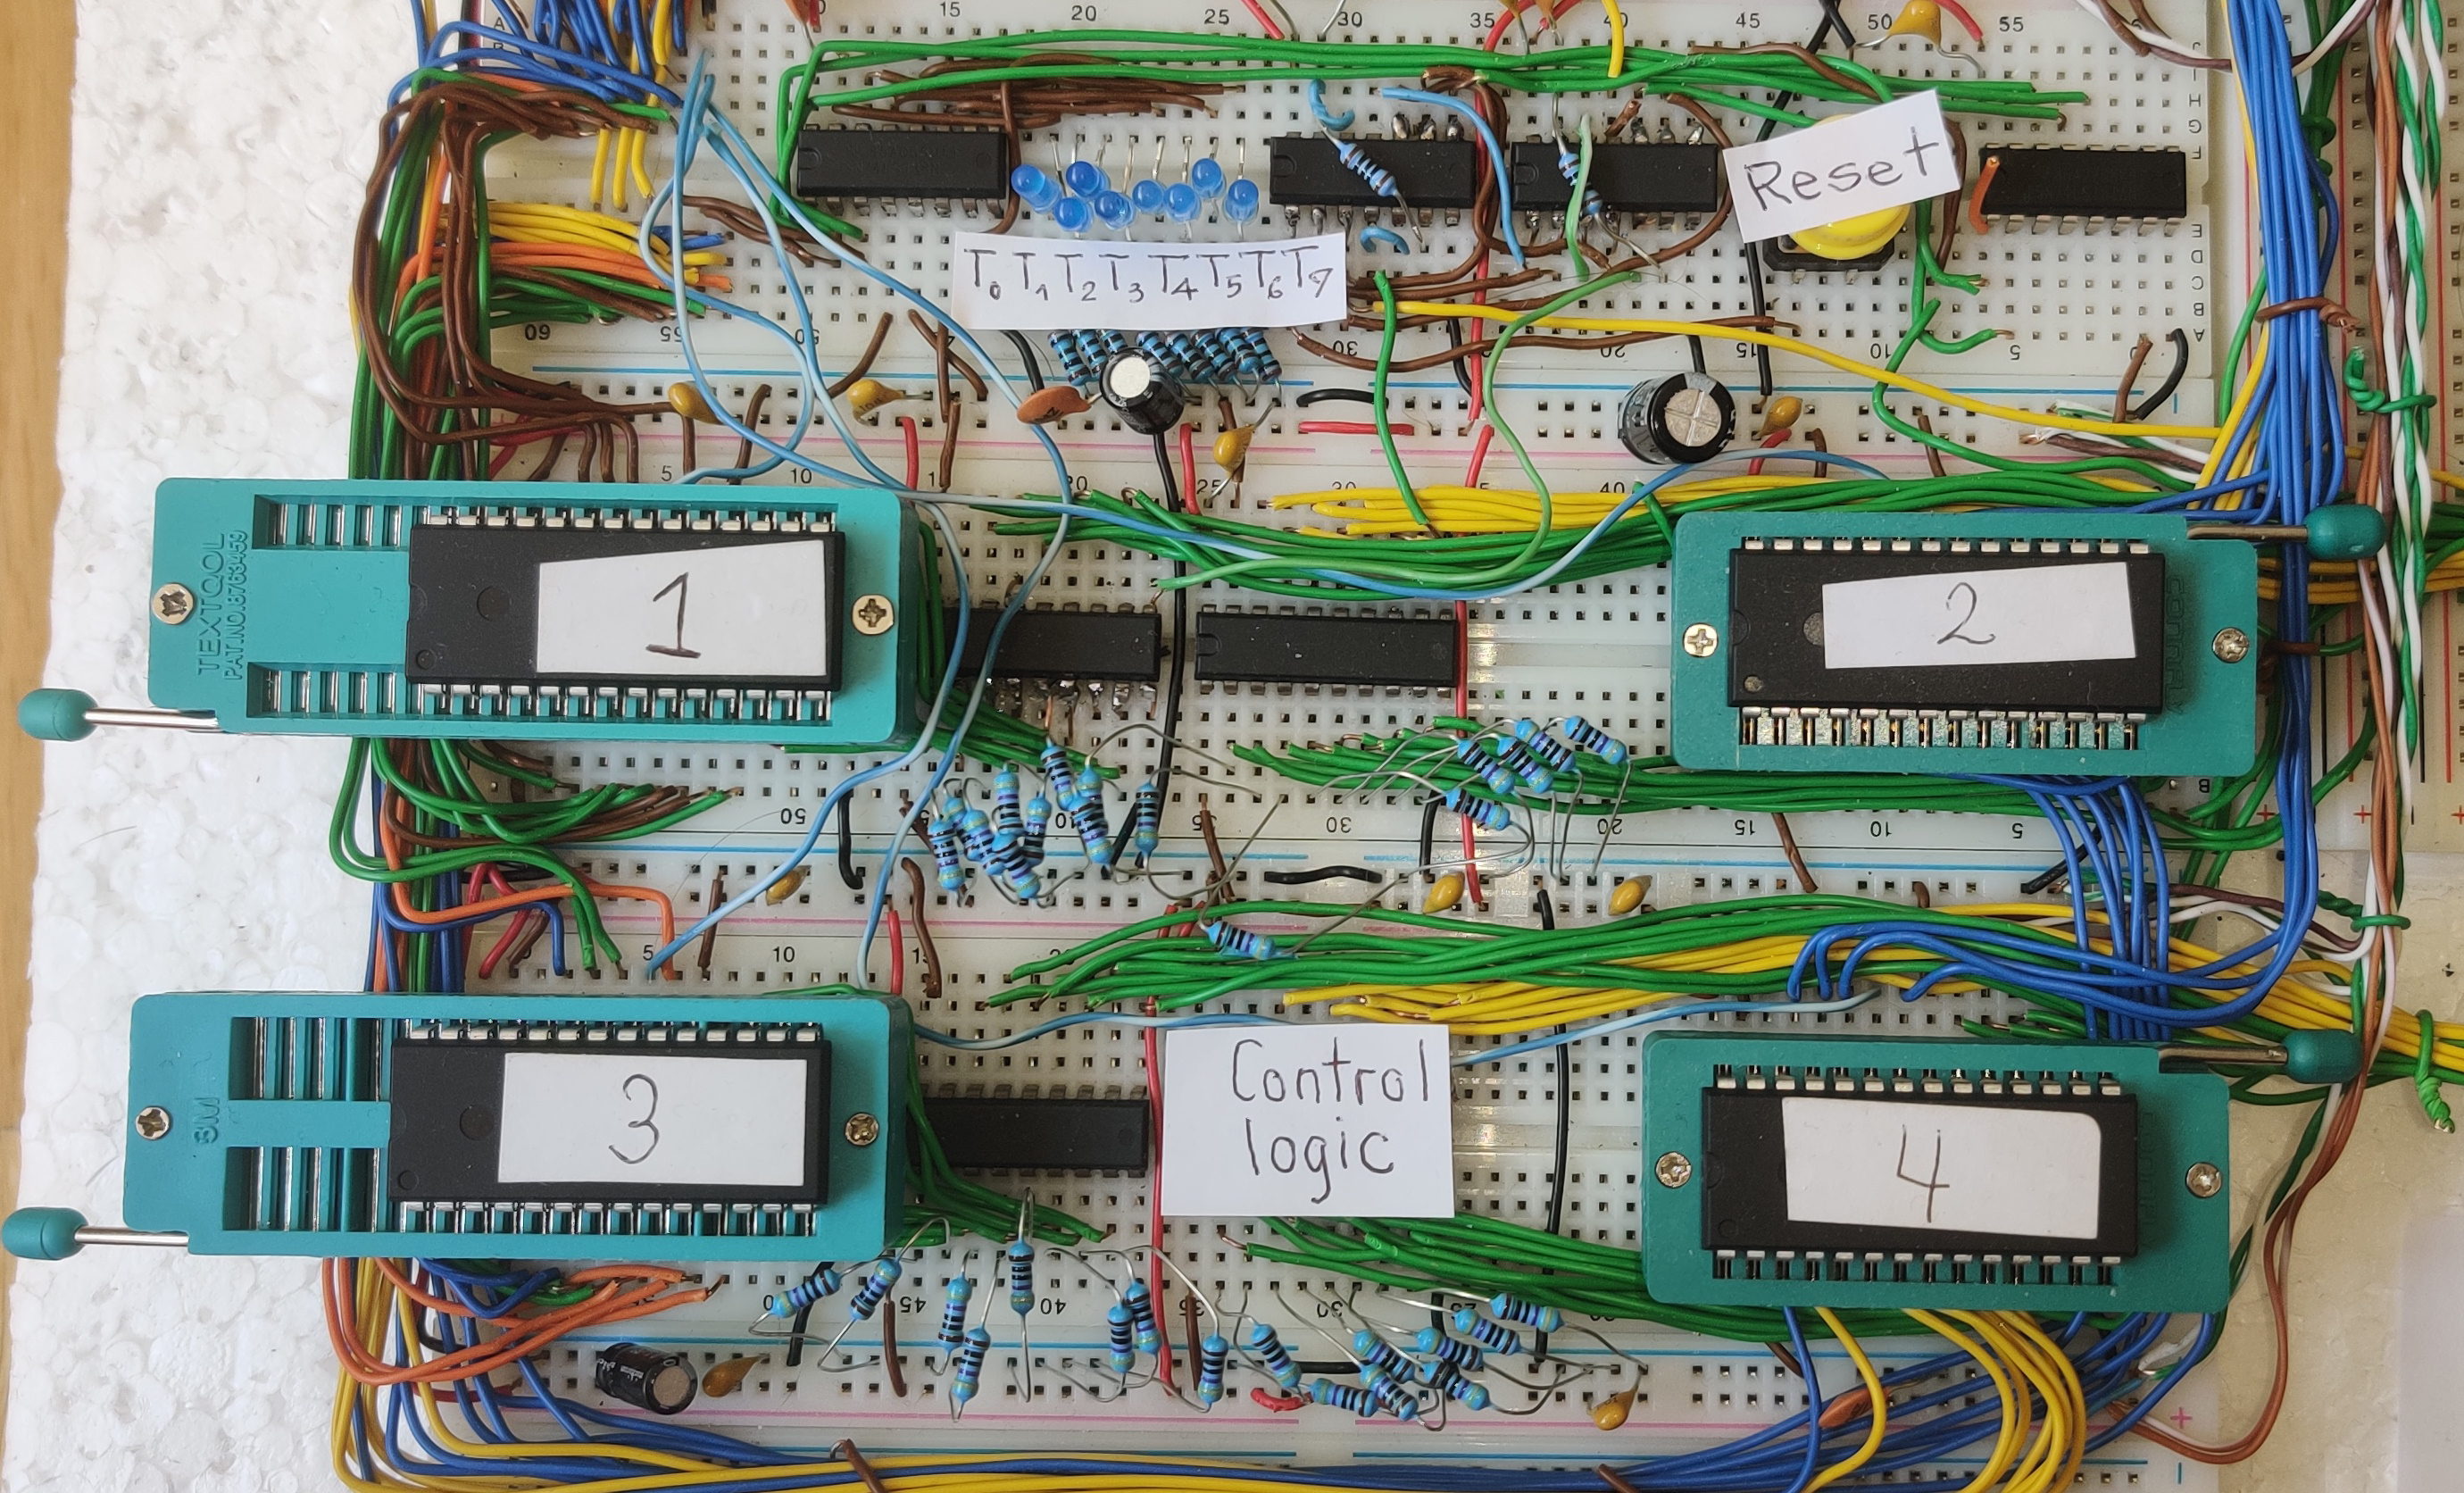
\includegraphics[scale=0.1]{comp/control-logic}
    \caption{Control Logic implementation}
    \label{control-logic-i}
  \end{figure}

  \begin{figure}[h]
    \centering
    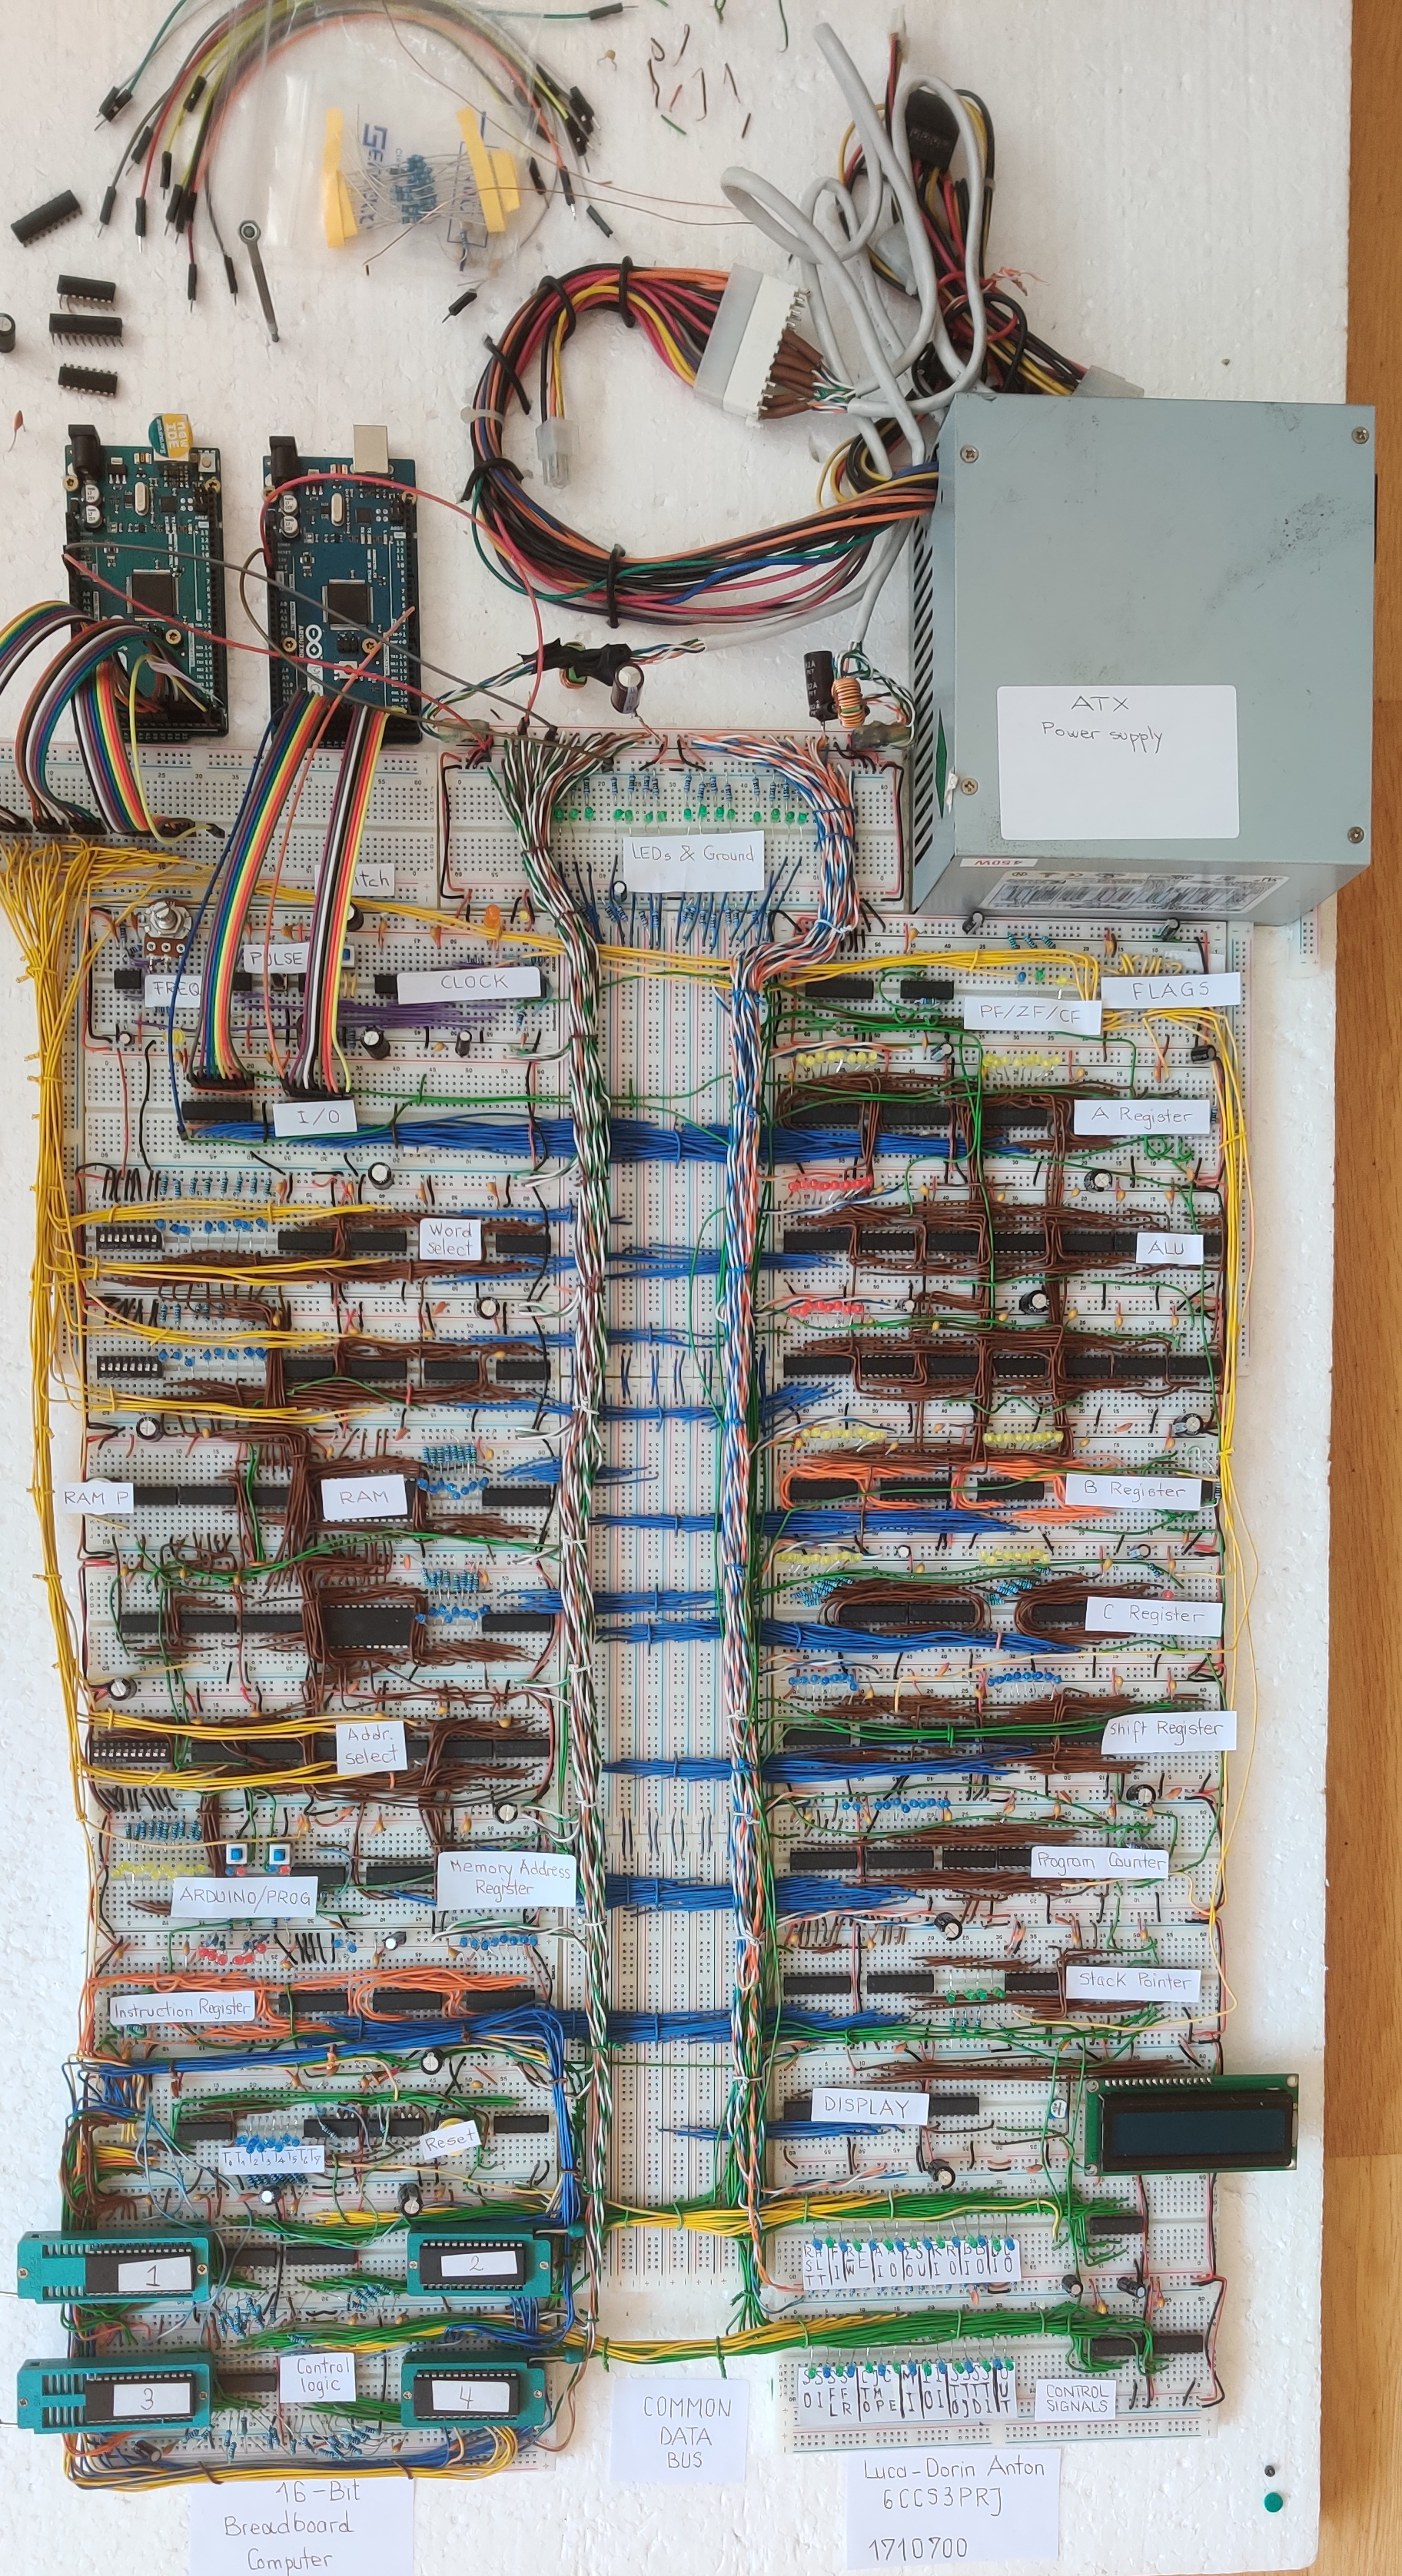
\includegraphics[scale=0.1]{comp/high-level}
    \caption{High level overview (with bus and LEDs visible)}
    \label{high-level-i}
  \end{figure}

\cleardoublepage
\cleardoublepage
